%\documentclass[10pt, twocolumn]{article}
%\documentclass[11pt]{article}
%\documentclass[twocolumn,showpacs,preprintnumbers,amsmath,amssymb,prl, superscriptaddress]{revtex4}
\documentclass[twocolumn,preprintnumbers,amsmath,amssymb,prl, superscriptaddress]{revtex4}
%\documentclass[preprintnumbers,amsmath,amssymb,prd,superscriptaddress]{revtex4}
%\documentclass[10pt, preprint,showpacs,preprintnumbers,amsmath,amssymb, superscriptaddress]{revtex4}
%\documentclass[11pt, prd,preprintnumbers,amsmath,amssymb, superscriptaddress]{revtex4}
%\documentclass[11pt, prd,preprintnumbers, amsmath,amssymb, superscriptaddress, nofootinbib, hyperref]{revtex4}


\usepackage{latexsym}
\usepackage{amssymb}
\usepackage{epsfig,amsmath,graphics}
\usepackage{epstopdf}
\usepackage{verbatim}
\usepackage{wasysym}
\usepackage{hyperref}
\usepackage{feynmp-auto} % feynman diagrams
%\usepackage{subfig}
\usepackage[utf8]{inputenc}
\usepackage{xpatch}
\usepackage{xcolor}
\hypersetup{
    colorlinks,
    linkcolor={red!80!black},
    citecolor={green!60!black},
    urlcolor={blue!60!black}
}
\usepackage{appendix}

\newcommand{\Ez}{\mathcal{E}_0}
\newcommand{\Eboom}{\mathcal{E}_\text{boom}}

\newcommand{\OO}{\mathcal{O}}
\newcommand{\LL}{\mathcal{L}}
\newcommand{\HH}{\mathcal{H}}

\newcommand{\TeV}{\text{TeV}}
\newcommand{\GeV}{\text{GeV}}
\newcommand{\MeV}{\text{MeV}}
\newcommand{\keV}{\text{keV}}
\newcommand{\rad}{\text{rad}}
\newcommand{\cm}{\text{cm}}
\newcommand{\angstrom}{\buildrel _{\circ} \over {\mathrm{A}}}
\newcommand{\pslash}{p\hspace{-0.070in}/\,}
\newcommand{\Mpl}{M_{\text{pl}}}
\newcommand{\ket}[1]{\ensuremath{\left|#1\right>}}
\newcommand{\bra}[1]{\ensuremath{\left<#1\right|}}
\newcommand{\braket}[2]{\ensuremath{\left<#1|#2\right>}}
%Large Parentheses
\def\r{\right)}
\def\l{\left(}

\begin{document}

%\preprint{APS/123-QED}


\title{White Dwarfs as Dark Matter Detectors}

\author{Peter W. Graham}
\affiliation{Stanford Institute for Theoretical Physics, Department of Physics,
Stanford University, Stanford, CA, 94305}

\author{Ryan Janish}
\affiliation{Berkeley Center for Theoretical Physics, Department of Physics,
University of California, Berkeley, CA 94720, USA}

\author{Vijay Narayan}
\affiliation{Berkeley Center for Theoretical Physics, Department of Physics,
University of California, Berkeley, CA 94720, USA}

\author{Surjeet Rajendran}
\affiliation{Berkeley Center for Theoretical Physics, Department of Physics,
University of California, Berkeley, CA 94720, USA}

\author{Paul Riggins}
\affiliation{Berkeley Center for Theoretical Physics, Department of Physics,
University of California, Berkeley, CA 94720, USA}

\begin{abstract}

White dwarfs can serve as detectors for ultra-heavy dark matter states which interact to trigger type Ia supernovae through thermonuclear runaway. 
This was originally proposed in \cite{Graham:2015apa} and used to place bounds on primordial black holes.
In this paper, we extend the reach of white dwarf detectors to dark matter candidates with non-gravitational couplings that release energy in the form of standard model particles.
This is used to constrain dark matter models which can ignite white dwarfs through annihilations, decays, or transits.
As a concrete example, we are able to constrain supersymmetric Q-ball dark matter in a vast region of parameter space fundamentally inaccessible to terrestrial-based experiments.


\end{abstract}
\maketitle
%\tableofcontents
%\newpage

\section{Introduction}
\label{sec:Introduction}

The existence of dark matter (DM) in the universe is strong evidence for physics beyond the Standard Model (SM).
Similar to the matter content in the SM, it is natural to suspect that the DM also has non-gravitational interactions.
Although there are many experiments designed to detect DM at the weak scale or lighter, these experiments are unable to probe ultra-heavy candidates that have too low a flux on terrestrial detectors. 
Even if the DM mean free path were smaller than the detector size, such interactions would be incredibly rare events. 
For instance, DM masses above $\sim 10^{22} ~\GeV$ will register fewer than a single event per year in a typical detector of surface area $\sim (100 ~\text{m})^2$.
Although such candidates are unlikely fundamental particles, in the presence of self-interactions it is natural to expect that the DM is able to form large composite states just as the SM produces complex structure of mass parametrically greater than the weak scale. 
One possibility to detect ultra-heavy DM proposed by \cite{Graham:2015apa} is that DM can trigger supernovae (SN) in sub-Chandrasekhar white dwarf (WD) stars by inducing runaway fusion.
As such, white dwarfs can serve as DM detectors. 

White dwarfs are particularly suited to this task as they are more susceptible to runaway fusion than are main-sequence stars.
Runaway fusion requires that two criteria be met: a region within the star must be hot enough to support exothermic fusion reactions, and the rate at which energy is released must dominate any cooling mechanisms that drain energy from the fusing region.
Since the pressure of a WD is set by electron degeneracy and is thus independent of temperature, thermal expansion is suppressed as a potential cooling mechanism.
Therefore WD cooling relies on thermal diffusion, which becomes less important over longer length scales, and can be overcome by sufficiently heating a large enough region of the WD.

The necessary trigger for runaway fusion was initially computed in \cite{Woosley} and recently implemented in \cite{Graham:2015apa} to place bounds on primordial black holes.
In addition, the authors of \cite{Graham:2015apa} identify several other heating mechanisms involving DM which may be constrained in a similar manner.
Here we extend the reach of WD detectors to DM candidates with non-gravitational couplings which release energy in the form of high-energy standard model (SM) particles.
DM models with interactions of this sort include Q-balls found in supersymmetric extensions of the SM and dark nuclei with higher-dimension couplings to the SM \cite{Hardy:2014mqa}.
An essential ingredient in this analysis is an understanding of how individual SM particles deposit energy in a WD medium through strong and electromagnetic interactions.
In this regard, the WD may be thought of as a detector with hadronic and electromagnetic ``calorimeter'' components.
This is used to constrain DM models which can ignite WDs via DM-DM collisions, DM decays, or transits with a DM-SM scattering interaction.
The proposed bounds will come from either observing specific, long-lived white dwarfs or comparing the measured type Ia SN rate with the expected rate due to DM events.
As a concrete example, we are able to constrain Q-ball DM in regions of parameter space fundamentally inaccessible to terrestrial experiments.
However, it is important to note that any such DM constraints are by nature complimentary to terrestrial ones - it is more massive DM that is likely to trigger SN, and also more massive DM that has sufficiently low flux on Earth.
What allows the WD detector to be effective in this regime is its enhanced surface area $\sim (10^4 ~\text{km})^2$, exceptionally long lifetime $\sim \text{Gyr}$, and astronomical abundance in the galaxy.

We begin in Section~\ref{sec:Review} by reviewing the mechanism of runaway fusion in a WD.
The ability for DM to trigger SN through non-gravitational interactions is ultimately based on the heating properties of ordinary SM particles, which is summarized in Section~\ref{sec:SMHeating} for different species and energies.
In Section~\ref{sec:DMexplode} we derive conditions on the properties of DM necessary to ignite white dwarfs, and in Section~\ref{sec:Constraints} we constrain DM models with interactions parameterized by a simple, schematic form.
We examine the specific case of Q-balls in Section~\ref{sec:QBalls}, and conclude in Section~\ref{sec:Discussion}.

\section{White Dwarf Runaway Fusion}
\label{sec:Review}

Any process which deposits energy in a WD will eventually heat a localized region within the star.
Since we are interested in nuclear fusion, let $L_0$ be the length scale of the local peak in ion temperature $T_0$ and $\Ez \sim n_\text{ion} T_0 L_0^3$ be the excess thermal energy it contains, where $n_\text{ion}$ is the number density of ions.
Note that the size and thermal properties of any heated region will evolve in time, so we take $L_0$ and $\Ez$ to characterize this peak as it initially forms, i.e.\ immediately after a temperature profile for ions has been established.
Thus for a given heating event, $L_0$ is a measure of the efficiency with which the energy deposit is transferred to ions in the stellar medium.
This may vary significantly with the form of the energy deposit and with WD density.
For example, suppose that kinetic energy is transferred directly to a single ion through a short-range elastic scatter.
This ion would thermalize with neighboring ions, resulting in a heating length $L_0$ of order the ion mean free path.
In the other extreme, suppose that a process produces electrons in the WD at energies just above the Fermi energy.
These electrons have Pauli-suppressed interactions and will travel a long distance before their energy is scattered and thermalized among ions, resulting in a much larger $L_0$.

The fate of a locally heated region in a WD is either a nonviolent diffusion of the energy deposit across the star, or a runaway fusion chain-reaction that will destroy the star.
The precise outcome is governed by two parameters: the fusion temperature $T_f$ and trigger size $\lambda_T$.
The fusion temperature $T_f$ is the threshold for the onset of fusion and is given by the energy required for ions to overcome their mutual Coulomb barrier.
For carbon-carbon fusion, this is of order $T_f \sim \MeV$ \cite{Gasques:2005ar}. 
However, while any region with $T_0 > T_f$ will initially support fusion, this condition is not sufficient for triggering a runaway process.
Sustained heating through nuclear fusion can only be maintained if the timescale for cooling is consistently longer than the timescale for heating.
Cooling in a WD is dominated by diffusion and the characteristic diffusion time for a heated region increases with its size while the rate of fusion is independent of size.
Therefore, there will always be a critical size of a heated region (at fixed temperature) above which fusion is maintained as the dominant thermal process.
For a region at the threshold of nuclear fusion $T_f$, this condition defines the trigger size $\lambda_T$.
The value of $\lambda_T$ is highly dependent on stellar density, and is set by either the thermal diffusivity of photons or degenerate electrons.
It has been calculated numerically in \cite{Woosley} and analytically scaled for varying WD masses in \cite{Graham:2015apa}.
As in \cite{Graham:2015apa}, we restrict our attention to carbon-oxygen WDs in the upper mass range $\sim 0.85 - 1.4 ~M_{\odot}$ which correspond to a central number density of ions $n_\text{ion} \sim 10^{30} - 10^{32} ~\cm^{-3}$ \cite{cococubed}.
Over this range, the trigger size is approximately $\lambda_T \sim 10^{-5} - 10^{-3} ~\text{cm}$.

In summary, a local temperature peak $T_f$ in a WD will either always be dominated by diffusive cooling if $L_0 < \lambda_T$ or sustained fusion if $L_0 > \lambda_T$.
However, there is an additional possibility if $T_0 > T_f$ that the thermal evolution is initially dominated by diffusion but at a later time results in runaway fusion.
We can assess this outcome by assuming the region with $T_0 > T_f$ begins to diffuse and cool until its temperature reaches $\sim T_f$.
If the size of the region at this point is larger than $\lambda_T$, a runaway will occur.
For a heated region of initial size $L_0$ and total energy deposit $\Ez$, the condition to trigger a type Ia SN via runaway fusion is
\begin{equation}
\label{eq:boom}
  \Ez \gtrsim n_\text{ion} T_f \text{max}\{L_0, \lambda_T\}^3.
\end{equation}
This implies the explosion condition used in \cite{Graham:2015apa}, but also provides a less stringent criteria applicable to regions of temperature greater than $T_f$ and size less than $\lambda_T$ which was not needed in that work.
Thus there is an absolute minimum energy required to ignite a WD
\begin{equation}
\label{eq:Eboom}
\mathcal{E}_{\text{boom}} \sim n_\text{ion} T_f \lambda_T^3 \sim 10^{15} - 10^{20} ~\GeV,
\end{equation}
where $\mathcal{E}_{\text{boom}} $ varies with trigger size $\lambda_T$ over the range of WD densities.
This is plotted in Figure \ref{fig:Eboom}.
Note that the threshold \eqref{eq:Eboom} is only sufficient if the deposited energy thermalizes within a region of size $L_0 < \lambda_T$.
The threshold energy for explosion is parametrically larger if energy is deposited on a larger length scale $L_0 > \lambda_T$.
As a result, understanding the heating length $L_0$ of a process is critical to determining whether or not it is capable of destroying a WD.
\begin{figure}
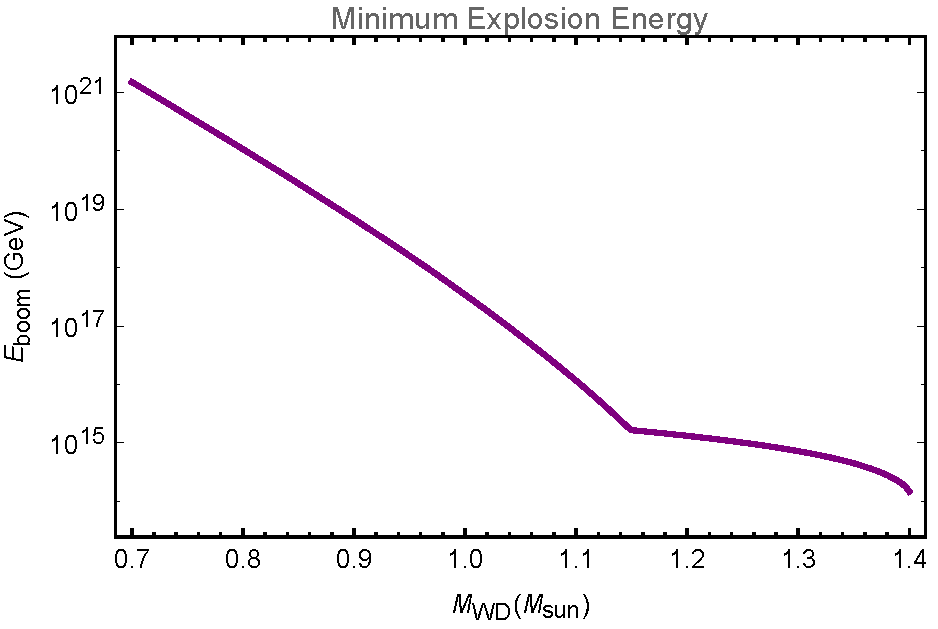
\includegraphics[scale=.45]{Eboom.pdf}
\caption{Minimum energy $\Eboom$ required to trigger SN as a function of WD mass, based on numerical results for $\lambda_T$ \cite{Woosley}.}
\label{fig:Eboom}
\end{figure}

\section{Non-Gravitational Heating of White Dwarfs}
\label{sec:SMHeating}

Having reviewed the requirements for runaway fusion in a WD, we turn to the question of triggering these events with DM.
This amounts to determining the heating length $L_0$ and energy deposit $\Ez$ due to a given DM encounter with a WD - if condition \eqref{eq:boom} is satisfied, then the encounter is explosive.
Of course, the parameters $L_0$ and $\Ez$ necessarily depend on the nature of the DM and must be explicitly calculated for a given DM model.
This was done in \cite{Graham:2015apa} in the case of primordial black holes, which deposit energy through dynamical friction while transiting the star.
However, non-gravitational interactions also have the potential to trigger SN.
In particular, any DM candidate which couples to the SM will generically be able to release SM secondaries which then thermalize with stellar constituents.
For these types of processes, the unknown DM physics serves only to determine the initial distribution in space, energy, and species of the SM particles produced in the star, while the actual heating proceeds entirely though known SM interactions.
It is therefore necessary to understand how energy is transferred from SM particles to the stellar medium in order to assess the explosiveness of these encounters.

The remainder of this Section is dedicated to computing the heating properties of SM species in a manner that is independent of the DM encounter.
We summarize here the dominant source of energy loss for each species while a more detailed treatment of particle interactions in a WD is reserved for Appendix \ref{sec:Appendix}.
Consider a schematic energy deposition in which $N$ particles of a single SM species and uniform energy $\epsilon$ are released isotropically in the stellar interior.
As we are primarily concerned with triggering runaway fusion, it is sufficient to take $\epsilon \gg T_f \sim \text{MeV}$.
In addition, either a few $N \sim 1$ ultra-high energy particles or a large number $N \gg 1$ of lower energy particles can be released.
These scenarios may have vastly different heating lengths, and we distinguish between the two when applicable.
The heating length of any such deposition is ultimately determined by the distances individual particles travel in a WD before giving up $\OO(1)$ of their energy.
This range can determined from the stopping power $(dE/dx)$ for different interactions, which is explicitly calculated in Appendix \ref{sec:Appendix}.
Subsequently, the resulting width of the initial ion temperature profile $L_0$ is computed for this schematic heating event in the case of light hadrons, electrons, photons, and neutrinos released in the WD.
It is important to note that if a process predominantly transfers energy to electrons or additional secondaries, the relevant length scale will be the larger distance over which \emph{ions} are eventually heated.

\subsection{Heating Properties: Hadrons}

For high-energy incident hadrons, the energy loss is dominated by inelastic nuclear collisions in which the incoming hadron violently interacts with a target nucleus to produce an $\OO(1)$ number of secondary hadrons.
This results in a roughly collinear hadronic shower that terminates when shower constituents reach a critical energy $E_\text{crit}$.
These final-state hadrons will consist of roughly equal fractions of pions, protons, and neutrons.
For neutrons, $E_\text{crit}$ is of order the nuclear binding energy $\sim 10 ~\text{MeV}$ although for charged hadrons, it is either $\sim 10 ~\MeV$ or the energy when Coulomb collisions with electrons becomes dominant.
The precise value of $E_\text{crit}$ is a nontrivial function of the WD density.
The shower length is determined by the typical mean free path $l_\text{inel}$ and cross-section $\sigma_\text{inel} \approx 100 ~\text{mb}$ for inelastic collisions:
\begin{align}
\label{eq:hadlength}
  X_\text{had} \sim l_\text{inel} \log\l\frac{\epsilon}{E_\text{crit}}\r
  \approx 10^{-6} ~\text{cm} \l\frac{10^{32}~\text{cm}^{-3}}{n_\text{ion}}\r.
\end{align}
As a result, a high-energy nucleon or pion ultimately transfers its energy to many low-energy hadrons, displaced a distance $X_\text{had}$ from its starting point.
Note that neutral pions decay to photons with a mean lifetime $\sim 10^{-16} ~\text{s}$, so that a $10 - 100 ~\text{MeV}$ neutral pion has a decay length of order $\sim 10^{-6} ~\text{cm}$.
Hence, there will be negligible electromagnetic contributions from $\pi^0$ decays during the progression of a hadronic shower.
For simplicity we focus on the hadronic component, which will carry a significant fraction of the shower energy.

At energies less than $\sim 10 ~\MeV$, protons and neutrons are predominantly stopped by elastic nuclear scatters, characterized by a mean free path $l_\text{el}$ and cross-section $\sigma_\text{el} \approx 1 ~\text{b}$.
On the other hand, charged pions will primarily transfer their energy to electrons in the stellar medium via Coulomb collisions.
Nevertheless, since each final-state nucleon and pion species carries $\OO(1)$ of the initial energy, a reasonable estimate of the heating length is obtained by considering only the final energy deposition from protons and neutrons.
We find that $\sim 10$ random-walk collisions are needed to slow $\sim 10 ~\MeV$ nucleons to $\sim \MeV$ energies, resulting in an elastic scattering distance of order
\begin{equation}
 \lambda_\text{el} \sim \sqrt{10} \times l_\text{el} \approx 10^{-7} ~\text{cm} \l\frac{10^{32}~\text{cm}^{-3}}{n_\text{ion}}\r
\end{equation}
If a single high-energy hadron $N \sim 1$ is released in the WD, the resulting ion temperature profile will be displaced from the origin by the hadronic shower length $X_\text{had}$ with characteristic size $L_0 \sim \lambda_\text{el}$.
If instead many hadrons $N \gg 1$ are initially released and thermalize collectively, the heating length will be of order $L_0 \sim X_\text{had} + \lambda_\text{el} \approx X_\text{had}$.
In either case, the heating length is parametrically smaller than the trigger size $\lambda_T$ and so the release of high-energy hadrons is an efficient heating mechanism for WDs.

\subsection{Heating Properties: Electrons and Photons}

We now consider the heating properties of electrons and photons together as their interactions are highly coupled.
In this case, the dependence on WD density is not as straightforward due to the LPM effect, which suppresses radiative processes at high densities.
We explicitly calculate the heating of a WD $n_\text{ion} \sim 10^{32} ~\cm^3$, although it is straightforward to generalize these results to lower densities - the only difference will be the turning points that characterize the dominance of one interaction over another.


At low energies, $\epsilon \lesssim 10~\GeV$, both electrons and photons primarily lose energy via elastic scattering off WD electrons.
Thus the first stage of heating will be to establish a region of heated electron gas.
Once the electrons equilibrate, they will begin to further lose energy via the previously sub-dominant bremsstrahlung process - this increases the photon number density, which transfers energy back into electrons by Compton scatters, and will eventually lead to the thermalization of the electrons and photon.
The establishment of this heated electron-photon gas will occur significantly before any energy is transfered to ions, as evidenced by the hierarchy between the electron-ion and photon-ion stopping powers and the election-photon stopping powers in Figure \ref{fig:SOMETHING}.
If the process originally released $N$ electrons or photons of energy $\epsilon \lesssim 10~\GeV$, then this electron-photon gas has a temperature of
\begin{align}
  T_{e\gamma} \sim \frac{N \epsilon}{Z n_\text{ion} \lambda_{e\gamma}^3}
\end{align}
where $\lambda_{e\gamma}$ is the range of electrons due to bremsstrahlung and we assume that $N$ is sufficiency large so that $T_{e\gamma} \gtrsim 1~\MeV$.

Note that if $T_{e\gamma} \lesssim 10~\MeV$, the only routes to transfer energy to ions are dramatically suppressed.
In that case, ion heating is dispersed over an insignificantly large region.
However, if $T_{e\gamma} \gtrsim 10~\MeV$, then photons in this gas will transfer their energy to ions via photonuclear scatters, which are nonelastic nuclear scatters as discussed in Section \ref{sec:SOMETHING} between a photon and a nucleus, mediated by a virtual quark pair.
As $N$ is large and each photon carries a small fraction of the total deposited energy, the effect here is to launch many hadronic showers from the electron-photon gas which heat ions as discussed.
The total length of these photo-nuclear showers is given by $l_\gamma + X_\text{had}$, where $X_\text{had}$ is the hadronic shower length and $l_\gamma$ the mean free path for a photonuclear collision, which is related to the hadronic mean free path for nonelastic nuclear collisions by $\sim l_\text{h,non}/\alpha$.
The photonuclear piece dominates, and it also dominates the initial scale of the heated electrons and photons $\lambda_{e\gamma}$, so we find that a low-energy cloud of electrons or photons will eventually heat ions over a distance $\sim l_\gamma$.

For slightly larger energies, there is a narrow window $10~\GeV \lesssim \epsilon \lesssim 100~\GeV$ in which both electrons and photons are dominated by radiative processes.
In this regime we thus have an EM shower, which terminated at energies of $\sim 10~\GeV$ into a cloud of electrons and photons, which thermalize as described above.
This is a collinear shower covering about a decade in energy, so its principle effect is to amplify the number of energetic particles by a factor of $10$ and to disperse them over an EM shower length (note that since many particles are necessary involved here, this is a broadening of the heating peak and not a displacement).
If $N$ electrons or photons are released with energy $\epsilon$ and create EM showers, the shower products with thermalize an electron-photon gas of temperature
\begin{align}
  T_{e\gamma} \sim \frac{10 N \epsilon}{Z n_\text{ion} X_\text{EM}^3}
\end{align}
where $X_\text{EM}$ is the length of the EM shower.
At these densities, the shower lengths are extended by the LPM effect and given by
\begin{align}
  X_\text{EM} \sim X_0 \l \frac{\epsilon}{E_\text{LPM}} \r^{1/2},
\end{align}
where $E_\text{LPM} \sim$ \textcolor{blue}{NUMBERS} and $X_\text{EM} \sim$ \textcolor{blue}{NUMBERS}. \textcolor{blue}{citation}
As above, if $T_{e\gamma} \gtrsim 10~\MeV$ this will produce photonuclear hadronic showers and heat the ions over a scale $l_\gamma$.

Finally, at high energies $\epsilon \gtrsim 100~\GeV$ a released photon or electron will deposit energy directly into hadronic showers without first thermalizing a region of electron-photon gas.
Effectively, electrons and photons at this energy behave qualitatively like hadrons, with the quantitative difference in that they require a slightly longer distance to initiate a hadronic shower.
The physics is the same as that discussed in Section \ref{sec:SOMETHING}, though we now must add a photonuclear or electronucler length scale to the shower length $X_\text{had}$.
For $100~\GeV \lesssim \epsilon \lesssim 1~\TeV$, the shower is always photonuclear, as a released electron is more likely to bremsstrahlung than scatter off a nucleus and that bremmed photon is then able to start a photonuclear shower.
For $\epsilon \gtrsim 1~\TeV$, however, released electrons will start hadronic showers directly by radiating a virtual photon which undergoes a photonuclear collision.
This slows the electron over a length scale $\sim 10~l_\gamma/\alpha \sim 10 l_\text{h,non}/\alpha^2 $.

\subsection{Heating Properties: Neutrinos}

Neutrinos interact very weakly, although their nuclear cross-section $\sigma_{\nu A}$ rises with energy.
At an energy of $\sim 10^{11} ~\GeV$, \cite{Formaggio:2013kya} calculates the cross-section to be $\sigma_{\nu A} \sim 10^{-32} ~\cm^2$.
Taking this to be a conservative estimate for nuclear cross-section at even higher energies, we find the mean free path for a neutrino-nuclei scatter is of order $\sim \text{meter}$.
However, if we consider the release of a single ultra-high energy neutrino, than this mean free path is simply a displacement of the eventual thermal profile.
In a nuclear interaction, $20 \%$ of the neutrino energy is transferred to the nucleus while the rest is transferred to produced electrons.
In this case, the energy deposited to the nucleus is sufficient to start a hadronic shower.
Therefore, a ultra-high energy neutrino behaves like a hadron and the neutrino heating length is simply $L_0 \sim X_\text{had}$.

\subsection{Summary of Standard Model Heating Channels}

\section{Dark Matter-Induced Ignition: Conditions}
\label{sec:DMexplode}

In this Section, we parameterize aspects of the DM-induced heating of WDs that are purely dependent on the nature of DM.
In particular, we derive explosion conditions on DM-WD encounters in terms of their heating lengths $L_0$ that determine whether or not they are capable of igniting the star.
This is done for the three illustrative examples depicted in Figure \ref{fig:feynman}: DM-DM collisions, DM decays, and DM transits.
\begin{figure}
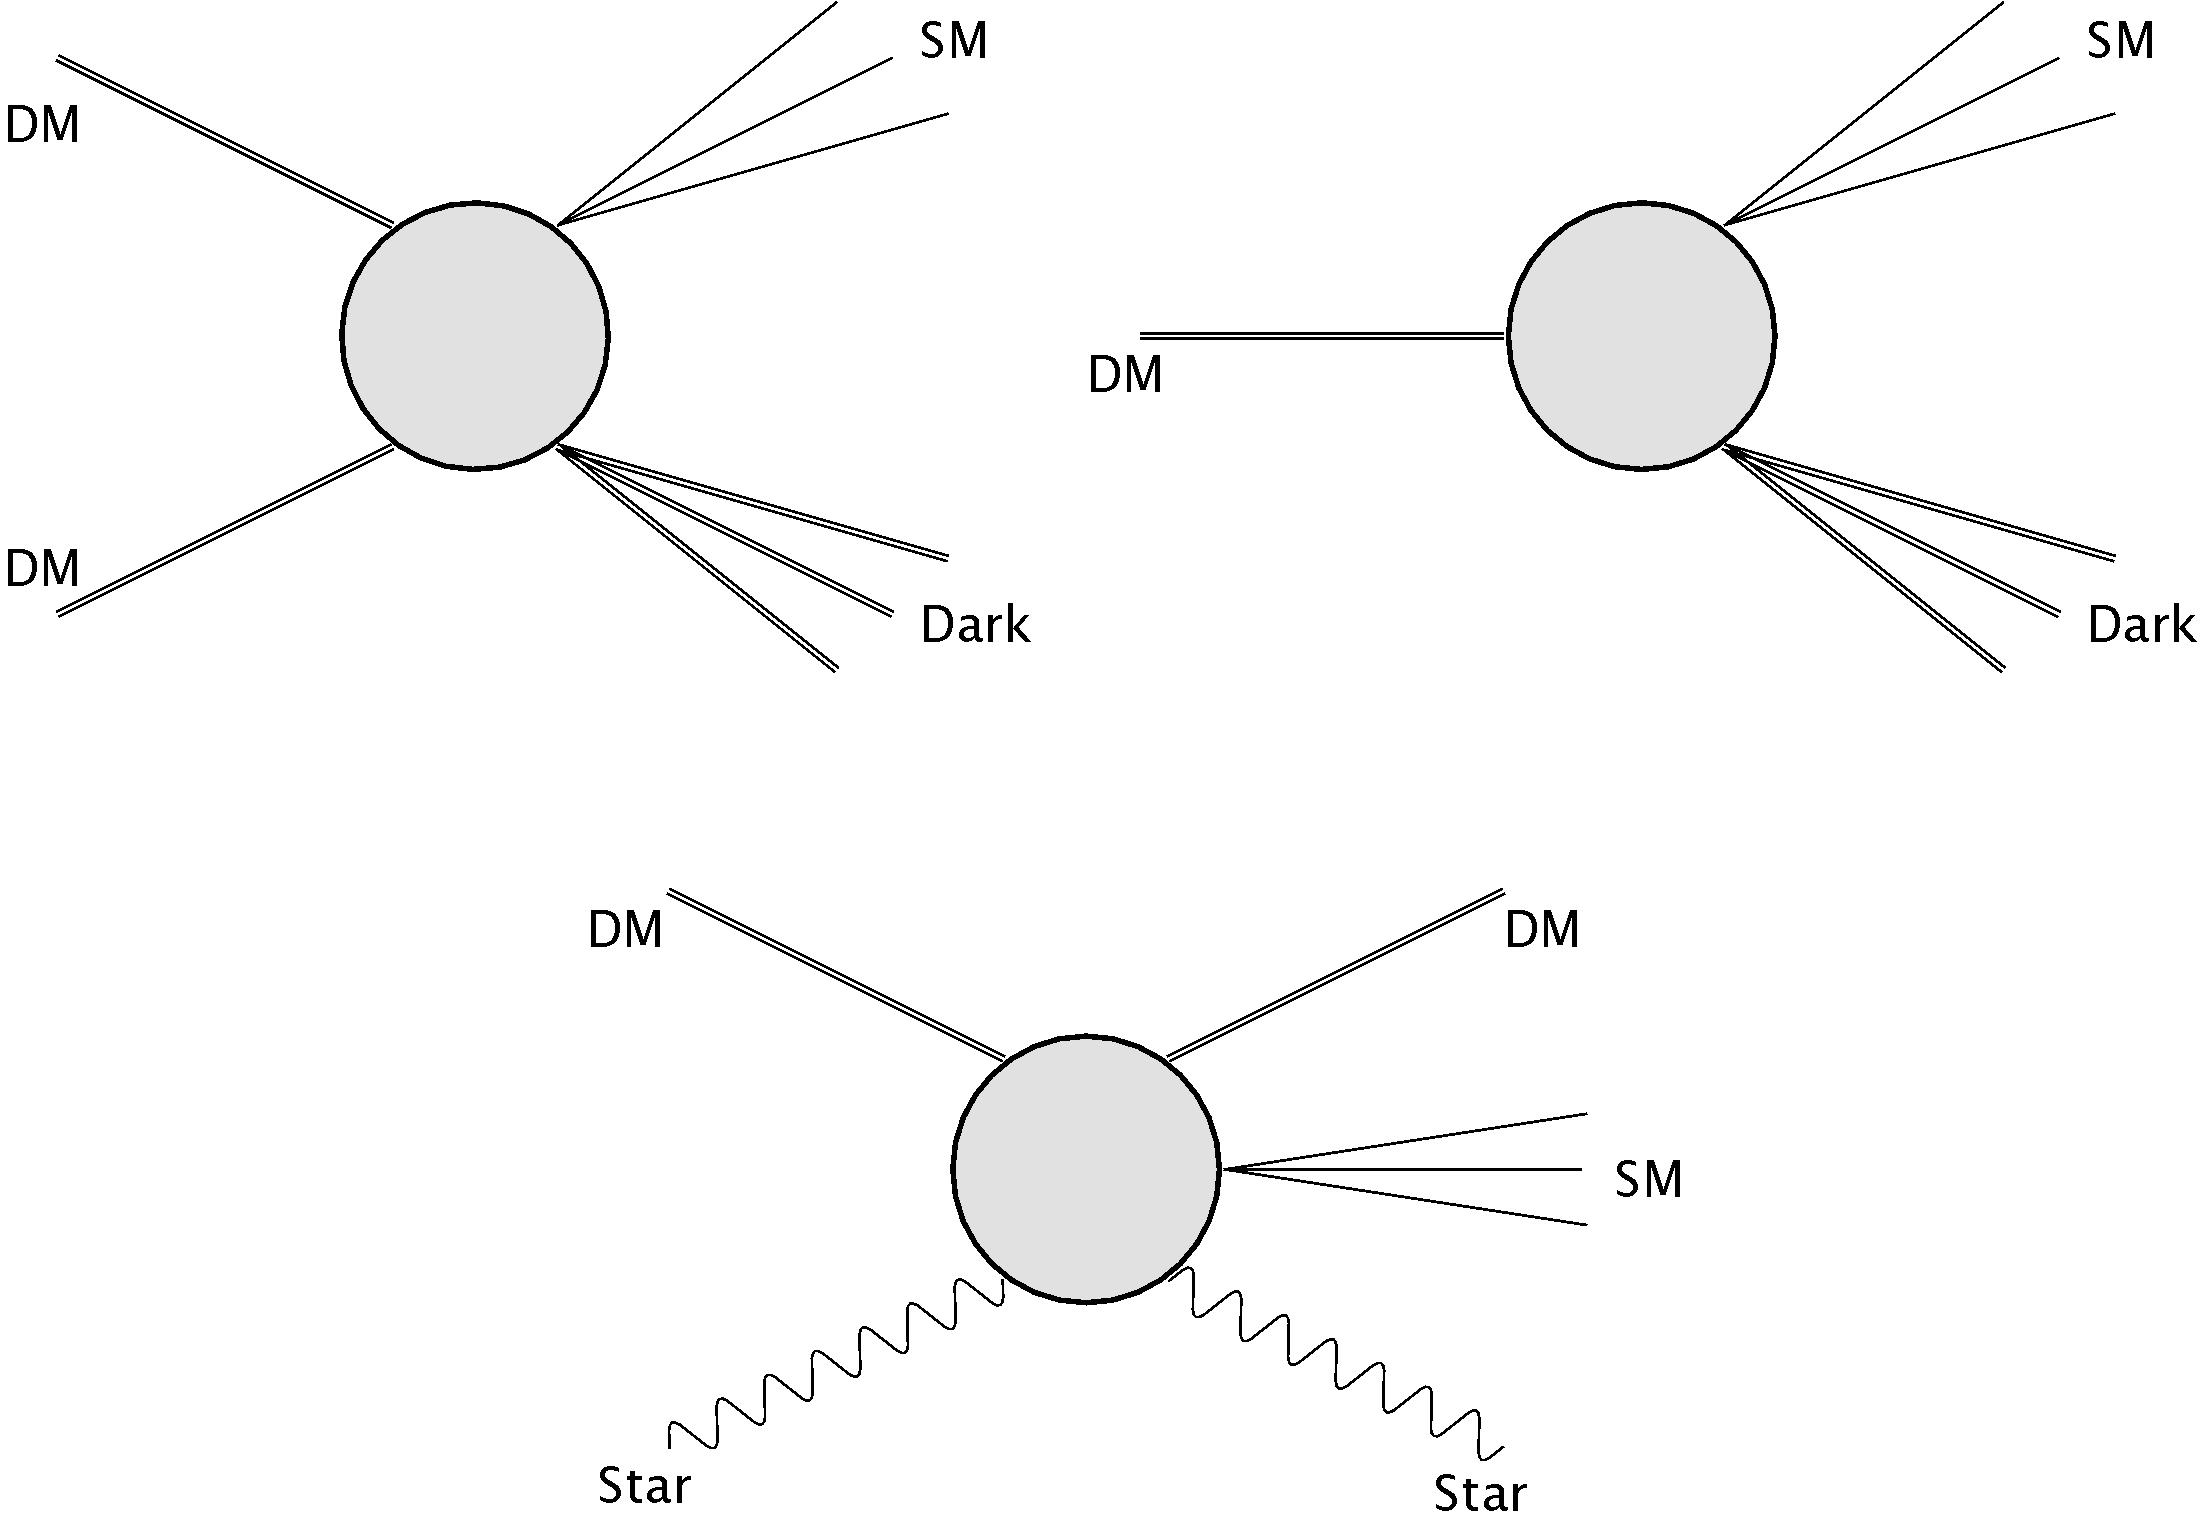
\includegraphics[scale=0.09]{feynmandiag.jpg}
\caption{Schematic of possible non-gravitational DM interactions in a WD. Heating of the WD occurs through SM particle production (also depicted are potential dark sector states involved).}
\label{fig:feynman}
\end{figure}

\subsection{DM-DM Collisions and DM Decays}
\label{sec:DMcoldecay}

The collision of two DM states or the decay of a single DM within the WD is a generic interaction found in many models.
Note that these DM-DM collisions are not necessarily particle-antiparticle annihilations, but can be of a more general, complicated nature such as the collisions of heavy nuclei.
Since any such event will likely result in both SM and dark sector products, we assume the energy released into the SM is a fraction $f_\text{SM}$ of the DM mass.
Generically we might expect $f_\text{SM} \ll 1$, although $f_\text{SM}$ is at most unity for non-relativistic DM.
For simplicity, we only consider ``point-like" annihilations and decays which release SM particles within a sufficiently localized region.
This excludes interactions involving the decay of long-lived, meta-stable dark states, i.e. displaced vertices.
With this parameterization, the explosion condition is approximately the same for both DM-DM collisions and DM decays:
\begin{equation}
\label{eq:coldecay}
  m_\text{DM} \gtrsim \frac{1}{f_\text{SM}} \cdot n_\text{ion} T_f \text{max}\{L_0, \lambda_T\}^3
\end{equation}
We are thus sensitive to ultra-heavy $(> 10^{15} ~\GeV)$ DM masses which annihilate or decay into SM particles. 

\subsection{DM Transits}
\label{sec:DMdecay}

For DM models with a DM-SM scattering interaction, there may be a continuous release of high-energy SM particles as the DM traverses a WD.
Since the DM will carry the bulk of the momentum in any such interaction producing light, relativistic SM secondaries, we can assume that the momentum of the released particles is isotropic.
This is parameterized by a linear energy transfer $(dE/dx)_\text{LET}$, which is the energy released into SM products per distance traveled in a WD.
Such a process can be broken up into a series of multiple heating events depositing energy $L_0 (d E/d x)_\text{LET}$ into temperature peaks of size $L_0$, where $L_0$ is the heating length for a single scatter.
If any individual deposition satisfies \eqref{eq:boom}, then runaway fusion obviously occurs.
If not, a SN may still be triggered due to the combined effect of many deposits.
In such a scenario a large number of nearby temperature peaks will each diffuse outward, eventually merging into an explosive thermal profile satisfying \eqref{eq:boom}.
This is possible if the heating length is smaller than the trigger size $L_0 < \lambda_T$, in which case it is sensible to consider the combined deposit as a single heating event of length $\lambda_T$ and energy $\lambda_T (d E/d x)$.
However, such a coherent addition of individual energy deposits is only possible if the DM transit time is smaller than the relevant thermal evolution timescale.
The latter is dominated by the diffusion time $\tau_d$ across a distance $\lambda_T$ at temperature $T_f$.
Thus we require
\begin{align}
\tau_d \sim \frac{\lambda_T^2}{\alpha(T_f)} \gg \frac{\lambda_T}{v_\text{esc}},
\label{eq:SlowDiffusion}
\end{align}
where $\alpha(T_f)$ is the temperature-dependent diffusivity.
This condition is independent of DM model and has been checked to be satisfied for all WD densities.

In addition, we can parametrize the DM kinetic energy loss per distance travelled in a WD by a DM stopping power $(dE/dx)_\text{SP}$.
Note that while $(dE/dx)_\text{LET}$ and $(dE/dx)_\text{SP}$ are conceptually related parameters and may be equal in important special cases, they are generically different.
We restrict ourselves to a ``bullet-like" transit in which DM penetrates the non-degenerate crust of a WD with negligible change in kinetic energy
\begin{align}
\label{eq:CrustCondition}
  \left( \frac{d E}{d x} \right)_\text{SP} \ll
  \frac{m_\text{DM} v^2_\text{esc}}{R_\text{crust}},
\end{align}
where $R_\text{crust} \sim 50 ~\text{km}$ is the width of a WD crust and $v_\text{esc} \sim 10^{-2}$ is the escape velocity of a WD.
If \eqref{eq:CrustCondition} were not satisfied, then the explosiveness of a transit would be highly dependent on details of the DM stopping power and must be calculated from a specific model.
We avoid this complexity by simply imposing that the DM reaches the degenerate stellar interior, where runaway fusion can be triggered, unimpaired in its initial transit of the star.
Furthermore, note that $R_\text{crust}$ is many orders of magnitude larger than $\lambda_T$ or any of the heating lengths considered in this work.
Therefore, the assumption of a DM transit at roughly constant velocity also allows us to ignore DM energy loss within the desired heating region in the WD interior.
The explosion condition for transits satisfying \eqref{eq:SlowDiffusion} and \eqref{eq:CrustCondition} is given by
\begin{equation}
\label{eq:transitexplosion}
  \left( \frac{d E}{d x} \right)_\text{LET} \gtrsim n_\text{ion} T_f\, \text{max}\left\{\lambda_T, L_0 \right\}^2.
\end{equation}

\section{Dark Matter-Induced Ignition: Constraints}
\label{sec:Constraints}

We now constrain models of DM which will ignite a WD via one of the processes parameterized in Section \ref{sec:DMexplode}.
In order to do so, we will additionally assume a simple, schematic form for the DM interaction such that the heating length of the encounter can be calculated explicitly. 
However, we first review the different ways in which white dwarfs can constrain DM candidates capable of triggering SN.

\subsection{Review of WD Observables}
Following the discussion of \cite{Graham:2015apa}, our constraints come from (1)~the existence of heavy, long-lived white dwarfs, or (2)~the measured type Ia SN rate.
The typical age of a WD is of order the age of the universe $\sim \text{Gyr}$.
RX~J0648.04418 is a nearby star and one of the heaviest known WDs with a mass $\sim 1.25 ~M_{\odot}$ \cite{Mereghetti:2013nba}.
Of course, this is not the only known heavy WD - the Sloan Digital Sky Survey \cite{SDSS} has found $\sim 20$ others.
The NuStar collaboration has also recently uncovered evidence for the likely existence of $\sim 1.25 ~M_{\odot}$ WDs in the galactic center as well \cite{NuStar}.
Such candidates are particularly suited for our constraints as the energy deposit necessary to trigger SN $\Eboom$ is a decreasing function of WD mass.
However, less dense white dwarfs are significantly more abundant in the galaxy.
Thus, even if a sufficiently massive DM is unable to trigger a violent heating event within the lifetime of a WD, it could still ignite enough lighter WDs to affect the measured SN rate of $\sim $ 0.3 per century.
The DM-induced SN rate is estimated using the expected number of white dwarfs per galaxy $\sim 10^{10}$ and their mass distribution \textcolor{blue}{cite}.
Simulations indicate that only WD masses heavier than $\sim 0.85 ~M_{\odot}$ will result in optically visible SN.
Therefore, most of the stars exploded in this manner will be in the mass range $\sim 0.85 - 1 ~M_{\odot}$, resulting in weaker SN than expected of typical Chandrasekhar mass WDs.

To summarize, a bound on DM parameters can be placed if either a single explosive event occurs during the lifetime of an observed star such as RX~J0648.04418, or the SN rate due to such DM events throughout the galaxy exceeds the measured value.
Note that for low-mass WDs dominated by photon diffusion, $\Eboom$ is a strong function of WD density.
In \cite{Graham:2015apa} the central WD density is used to constrain black hole transits with the justification that the density is nearly constant for much of the star.
The average density for WDs is typically a factor of $\sim 10^{-2} - 10^{-1}$ less than the central density, although it is found that the WD density changes by an $\OO(1)$ fraction from the central value out at a distance $\sim R_\text{WD}/2$ \cite{Chandrasekhar}.
Therefore the central density is a valid approximation as long as we consider heating events within this ``modified" WD volume.
For simplicity, we employ this approach


\subsection{Collision and Decay Constraints}
\label{sec:CollisionConstraints}

We begin by calculating the rate for a DM-DM collision or DM decay event to occur within the WD.
Note that it is possible that the DM has sufficient interactions with the SM capable of slowing it down in the WD.
If we consider such interactions, then there are two limiting behaviors: the DM enters the star at velocity $v_\text{esc}$ and exits with only an $\OO(1)$ change in its kinetic energy (``DM wind" scenario), or the DM gets stopped and accumulates (``DM capture" scenario) inside the WD.
The precise behavior is determined by the magnitude of the stopping power $(dE/dx)_\text{SP}$ relative to the quantity $m_\text{DM} v_\text{esc}^2/R_\text{WD}$. 
For any realistic models, it is reasonable to suspect that $(dE/dx)_\text{SP}$ is a strong function of DM velocity.
Therefore, we restrict ourselves to the two extreme cases of either negligible stopping or complete stopping of the DM. 
For DM wind, the expected number density of DM particles in the WD volume is simply
\begin{equation}
n_\text{DM} \sim \frac{\rho_{\text{DM}}}{m_\text{DM}} \frac{v_\text{esc}}{v},
\end{equation}
taking into account the $\OO(10)$ gravitational enhancement of the number density in the star. 
Here $v \sim 10^{-3}$ denotes the galactic virial velocity and $\rho_\text{DM}$ is the energy density of DM in the region of interest. 
We assume $\rho_\text{DM} \sim 0.4 ~\GeV/\text{cm}^3$ for nearby stars, while for the white dwarfs observed in the galactic center it is estimated that $\rho_\text{DM} \sim 10^3 ~\text{GeV}/\text{cm}^3$ \cite{Nesti:2013uwa}.
However, in the case of DM capture the number density of DM particles in the WD is dramatically increased due to the exceptionally long lifetime $\sim \text{Gyr}$ of the WD - as a comparison, the unstopped DM wind will spend of order $v_\text{esc}/R_\text{WD} \sim 1 ~\text{s}$ in the WD.
We find that the enhanced number density as a result of accumulation over a WD lifetime $\tau_\text{WD}$ is of order  
\begin{equation}
n_\text{DM} \sim \l \frac{\rho_\text{DM}}{m_\text{DM}} \r R_\text{WD}^2 \tau_\text{WD} \l\frac{v_\text{esc}^2}{v}\r.
\end{equation}
Although exact kinematics and stopping of the DM must be computed for a given model and $(dE/dx)_\text{SP}$, it is reasonable that the captured DM thermalizes to the WD temperature $T \sim \keV$ in a timescale shorter than the WD lifetime. 
Therefore, we can compute the expected DM-DM collision rate parameterized by cross-section $\sigma_\text{col}$
\begin{equation}
\Gamma_\text{collision} \sim n_\text{DM}^2 \sigma_\text{col} v_\text{DM} R_\text{WD}^3,
\label{eq:collisionDM}
\end{equation}
where $v_\text{DM}$ is the DM velocity in the WD and is either $\OO(v_\text{esc})$ for DM wind or $\OO(\sqrt{T/m_\text{DM}})$ for DM capture.
Likewise, the rate at which a single DM decay event occurs in the WD parametrized by a mean lifetime of DM $\tau_\text{DM}$ is simply
\begin{equation}
\Gamma_\text{decay} \sim  \frac{1}{\tau_\text{DM}} n_\text{DM} R_\text{WD}^3,
\label{eq:taugamma}
\end{equation}

We are able to constrain DM parameters whenever such processes satisfy the explosion condition $\eqref{eq:coldecay}$.
Consider a schematic interaction where an annihilation or decay releases a number of SM particles $N_i$ of single species $i$ and individual energy $\epsilon$. 
If we assume a fractional parameter $f_\text{SM}=1$, this corresponds to the entire mass of DM being converted into SM products $i$, each with energy $m_\text{DM}/N_i$.
These will deposit their energy and thermalize ions within a distance explicitly calculated in Section \ref{sec:SMHeating}. 
The only caveat is that the computed interactions of SM particles extrapolated to energies beyond the Planck scale must be done with caution as gravitational effects may become important. 
As a result, to adequately place constraints on ultra-heavy DM above this scale one can simply restrict the interactions to annihilations/decays into $N_i \gg 1$ particles of energy $\epsilon < 10^{18} ~\GeV$. 

It is important to note that there are additional limits on DM interactions of this kind, complementary to the limits placed from WDs. 
For instance, DM can annihilate or decay into ultra-high energy particles within our galactic halo and therefore contribute to the cosmic ray flux seen in terrestrial air shower detectors.
As we have not seen any cosmic rays of energy greater than $\sim 10^{12} ~\GeV$ \cite{ThePierreAuger:2015rha, AbuZayyad:2012ru}, this places a concrete limit on the DM interaction parameters $\sigma_\text{col}$ and $\tau_\text{DM}$ when such ultra-high energy particles are released. 
In theory, a constraint may also be placed on lower-energy SM products from DM annihilations or decays which would provide an additional source for the measured cosmic ray flux, although such a detailed analysis is beyond the scope of this work. 
The expected cosmic ray flux due to a DM decay in the galactic halo is given by:
\begin{equation}
\Gamma_\text{earth} \sim \int_{\text{halo}} \frac{\rho_\text{DM}(r)}{m_\text{DM}} \frac{R_\text{det}^2}{L^2} \frac{1}{\tau_\text{DM}},
\end{equation}
where $R_\text{det}^2 \sim (100 ~\text{km})^2$ denotes the typical surface area of a terrestrial cosmic ray detector and $L$ is the distance from the DM decay event to the earth. 
$\rho_\text{DM}$ is the expected density profile of DM throughout the galactic halo.
This integral can be calculated numerically using an NFW profile fit (as given by \cite{Nesti:2013uwa}) and the known distance from the earth to the center of the galaxy, although to a very good approximation the result is the same if we simply set the galactic parameters to the average values $\rho_\text{DM} \sim 0.4 ~\GeV/\cm^3$ and $L \sim R_\text{halo} \approx 50 ~\text{kpc}$. 
The constraint on DM is derived by requiring that the expected time for an event to strike earth $\Gamma_\text{earth}^{-1}$ is less than the lifetime of the detector $\sim 10 ~\text{yr}$.
Curiously, we find that in the case of DM decays the resulting bounds are of the same magnitude as those due to the observation of a local WD. 
This coincidence can be seen explicitly by comparing the effective ``space-time volume" for the two detectors.
A cosmic ray detector sees events within a space-time volume $\sim (R_\text{det}^2 R_\text{halo} \times 10 ~\text{yr})$ which is numerically similar to the WD space-time volume for decay events $\sim (R_\text{WD}^3 \times 10 \times 10^9 ~\text{yr}$), where the additional $\OO(10)$ factor is due to the gravitational Sommerfeld enhancement. 
Note that a similar calculation can be done in the case of DM-DM annihilations in the galactic halo, although in this case the gravitational enhancement is $\OO(10^3)$ and results in more stringent constraints from the WD observation. 

In addition, there are various cosmological bounds on DM interactions. 
By requiring that the galactic halo has not diminished by more than an $\OO(1)$ factor during its lifetime, we can constrain $\sigma_\text{col}/m_\text{DM} \lesssim \text{barn}/\GeV$, valid regardless of the precise details of the collision. 
The cosmological bound on DM lifetime $\tau_\text{DM} \gtrsim 100 ~\text{Gyr}$ is also independent of the nature of the decay products (see \cite{Poulin:2016nat} for details). 
Note that a similar bound on DM self-interactions $(\sigma_\text{col}/m_\text{DM})$ due to colliding clusters of galaxies \cite{Randall:2007ph} is of the same order of magnitude as that derived considering our own galaxy.
Since the limits imposed by the WD scale as $\sigma_\text{col} \propto m_\text{DM}^2$ and $\tau_\text{DM} \propto m_\text{DM}^{-1}$, there will necessary be a sufficiently large DM mass for which the above cosmological considerations are the more stringent constraints on its interactions. 
Lastly, we comment on the possibility for DM-DM collisions to affect the epoch of recombination and the observed properties of the cosmic microwave background (CMB). 
This effect was first computed in \cite{Padmanabhan:2005es} to constrain DM annihilations into products that inject energy to the photon-baryon plasma and ionize neutral hydrogen and is of the form $\langle \sigma_{col} v \rangle \propto m_\text{DM}$. 
Therefore, this could potentially be scaled to ultra-heavy DM masses if the cosmological history of such DM candidates is understood.

With the above schematic for DM-DM collisions, we place bounds on the cross section $\sigma_\text{col}$ as a function of $m_\text{DM}$ using the different classes of observation available and for representative choices of $f_\text{SM}$ and SM species $i$ released.
This is done in Figures \ref{fig:collisionclasses}, \ref{fig:collisioneta}, and \ref{fig:collisionspecies}. 
In a similar manner, we constrain the lifetime $\tau_\text{DM}$ as a function of $m_\text{DM}$ in Figures \ref{fig:decayclasses}, \ref{fig:decayepsilon}, and \ref{fig:decayspecies}.


\begin{figure}
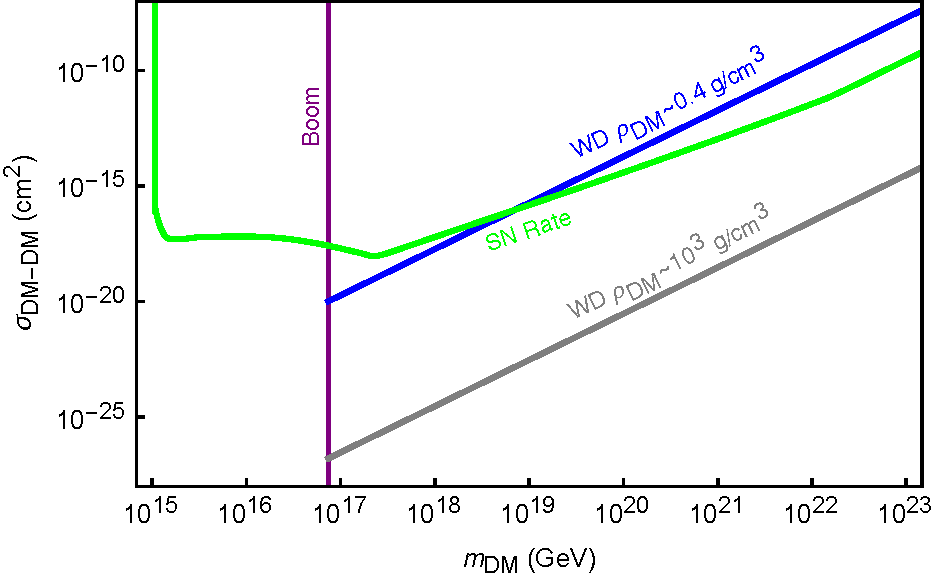
\includegraphics[scale=.45]{collisionobservation.pdf}
\caption{Constraints on DM-DM collision cross-section into photons with $f_\text{SM} =1$. Bounds come from observations of a single WD (local and galactic center) and measured SN rate}
\label{fig:collisionclasses}
\end{figure}

\begin{figure}
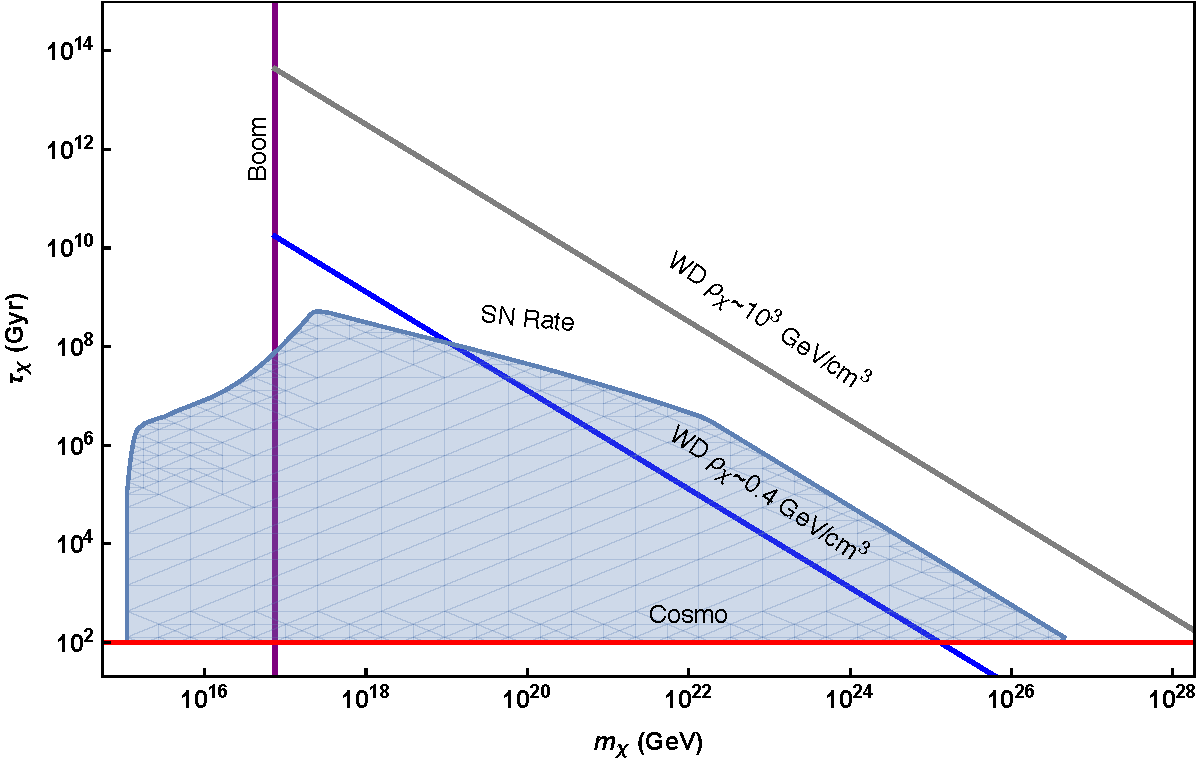
\includegraphics[scale=.45]{decayobservation.pdf}
\caption{Constraints on DM decay lifetime into photons with $f_\text{SM} =1$. Bounds come from observations of a single WD (local and galactic center) and measured SN rate}
\label{fig:decayclasses}
\end{figure}

\subsection{Transit Constraints}
\label{sec:TransitConstraints}

The DM transit rate through a WD (including a gravitational Sommerfeld enhancement) is given by
\begin{align}
\Gamma_\text{transit} \sim \frac{\rho_{\text{DM}}}{m_\text{DM}} R_\text{WD}^2 \l\frac{v_\text{esc}}{v}\r^2 v.
\label{eq:TransitFluxCondition}
\end{align}
In order to constrain a DM model through its transit interaction with a WD, we require that it satisfy the explosive condition \eqref{eq:transitexplosion}.
This is given in terms of an LET, which parameterizes the ability for DM to release sufficient energy to the star in the form of SM particles.
$(dE/dx)_\text{LET}$ for any realistic DM model would necessarily involve a sum over stellar targets along with species that could be produced, as well as an integral over the produced particle spectrum.
However, consider a simplified interaction in which $\sigma_{i,\epsilon}$ denotes the cross-section for DM to scatter off a stellar constituent, producing a particle of species $i$ and and energy $\epsilon$.
If this were the only available channel for the DM to deposit energy, then the LET could be written as
\begin{align}
\label{eq:schematicLET}
  \left( \frac{d E}{d x} \right)_\text{LET} = n_\text{ion} \sigma_{i,\epsilon} \epsilon,
\end{align}
where we now specify to the case of DM collisions with nuclear targets.
Assuming such a DM-SM scattering interaction, the transit heating length is computed in Section~\ref{sec:SMHeating}.

In addition, we also make a sensible assumption that the LET $(dE/dx)_\text{LET}$ and DM stopping power $(dE/dx)_\text{SP}$ are equal for fixed number density - that is, the DM loses kinetic energy at the same rate as energy is deposited to the WD.
While such a statement is certainly not true for all DM models (such as the Q-ball, which liberates binding energy rather than transferring kinetic energy), it provides a useful benchmark to express constraints.
With this assumption, it is interesting to note that combining the transit explosion condition \eqref{eq:transitexplosion} with $\eqref{eq:schematicLET}$ yields a lower bound on DM mass such that the DM is able to both penetrate the crust \emph{and} trigger an explosion:
\begin{align}
\label{eq:transitmass}
m_{\text{DM}} >  T_f \lambda_T^2 \l \frac{n_{\text{crust}} R_{\text{crust}}}{v_{\text{esc}}^2} \r.
\end{align}
For typical WD parameters we find that the DM mass must be greater than $\sim 10^{27} ~\GeV$, taking the density of the WD crust $n_\text{crust}$ to be a nominal $\OO(10^{-2})$ fraction of the central density $n_\text{ion}$ \cite{Chandrasekhar}.
In other words, if \eqref{eq:transitmass} were violated then the DM interaction is either not strong enough to ignite the WD or is so strong that the DM cannot penetrate the crust without losing appreciable kinetic energy.
However, it is important to note that this bound is only applicable when the energy input to the WD is chiefly coming from the DM kinetic energy, rather than binding energy or other sources.
With the above schematic for a DM transit, we constrain the parameter $\sigma_{i,\epsilon}$ as a function of DM mass $m_\text{DM}$.
This is done in Figures \ref{fig:transitclasses}, \ref{fig:transitepsilon}, and \ref{fig:transitspecies} using the different classes of observation available and for representative choices of $\epsilon$ and SM species $i$ released.

\begin{figure}
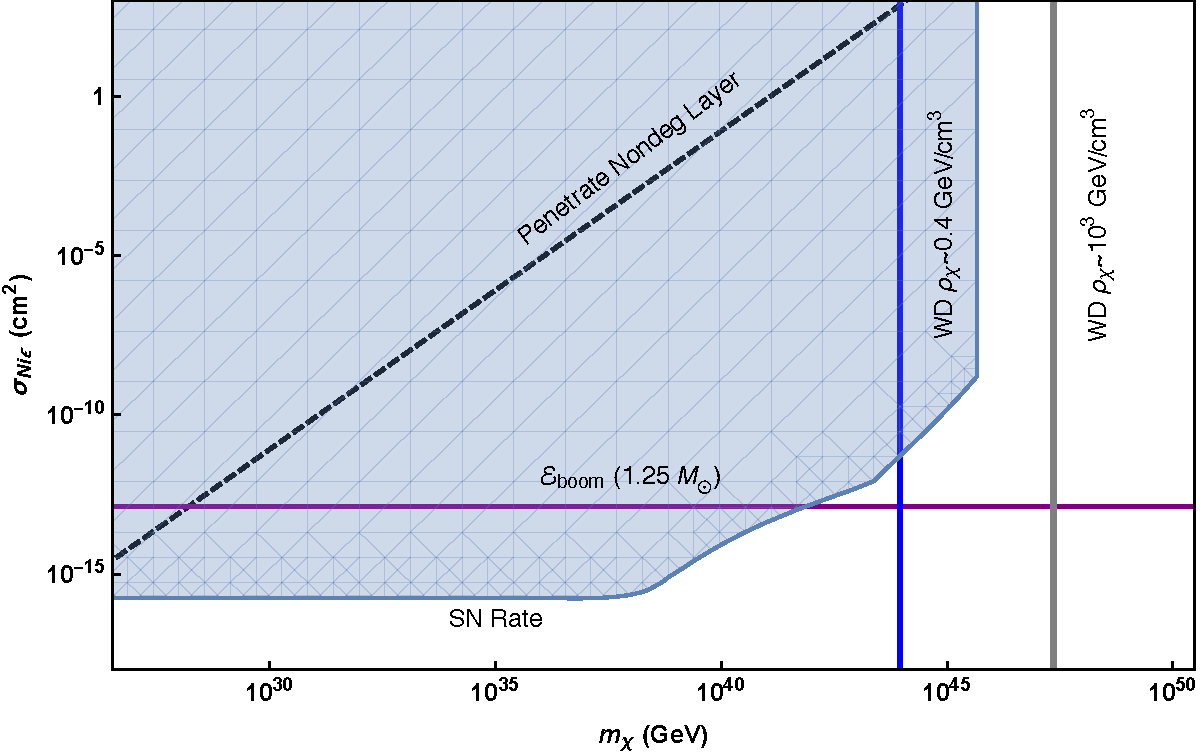
\includegraphics[scale=.45]{transitobservation.pdf}
\caption{Constraints on DM-nuclei scattering cross-section to produce photons of energy $\epsilon = \text{TeV}$. Bounds come from observations of a single WD (local and galactic center) and measured SN rate}
\label{fig:transitclasses}
\end{figure}

\section{Q-balls}
\label{sec:QBalls}

Having derived generic constraints on models of ultra-heavy DM in Section~\ref{sec:Constraints}, we turn towards a more concrete example: Q-balls.
In various supersymmetric extensions of the SM, non-topological solitons called Q-balls can be produced in the early universe \cite{Coleman:1985ki, Kusenko:1997si}.
If these Q-balls were stable, they would comprise a component of the DM today.
For gauge-mediated models with flat scalar potentials, the Q-ball mass and radius are given by
\begin{equation}
\label{eq:Qballprop}
M_Q \sim m_S Q^{3/4}, ~~~ R_Q \sim m_S^{-1} Q^{1/4},
\end{equation}
where $m_S$ is related to the scale of supersymmetry breaking.
The condition $M_Q/Q < m_p$ ensures that the Q-ball is stable against decay to nucleons \cite{Dine:2003ax}.
When an (electrically neutral) baryonic Q-ball interacts with a nucleon, it absorbs its baryonic charge as a minimum-energy configuration and induces the dissociation of the nucleon into free quarks.
During this proton decay-like process, $\sim \text{GeV}$ of energy is released through the emission of 2 - 3 pions \cite{Dine:2003ax}.
We assume that for each Q-ball collision, there is equal probability to produce $\pi^0$ and $\pi^\pm$ under the constraint of charge conservation.
The cross-section for this interaction is approximately geometric:
\begin{align}
\sigma_Q \sim \pi R_Q^2.
\end{align}
Note that a sufficiently massive Q-ball will become a black hole if the Q-ball radius is less than the Schwarzschild radius $R_Q \lesssim G M_Q$.
In the model described above, this translates into a condition $(M_\text{pl}/m_S)^4 \lesssim Q$.
For Q-ball masses of this order, gravitational interactions become relevant.

We now determine the explosiveness of a Q-ball transit.
As in Section \ref{sec:Constraints}, this process is described by the parameter
\begin{equation}
\l\frac{dE}{dx}\r_\text{LET} \sim n_\text{ion} \sigma_Q N \epsilon,
\end{equation}
where the nuclear collision results in $N \sim 30$ pions released, each with kinetic energy $\epsilon \sim 500 ~\text{MeV}$.
The Q-ball interaction is simple enough that the heating length of a Q-ball transit is computed in a straightforward manner $L_0 \approx 10^{-6} ~\text{cm}$ at a number density $n_\text{ion} \sim 10^{32}~\text{cm}^{-3}$.
$L_0$ scales inversely with $n_\text{ion}$ and is less than $\lambda_T$ for all WD densities.
Therefore, the Q-ball cross-section necessary to trigger runaway fusion is given by
\begin{equation}
\sigma_Q \gtrsim \lambda_T^2 \l \frac{T_f}{\epsilon}\r \approx 10^{-4} \lambda_T^2.
\end{equation}
If the Q-ball cross-section is related to its mass and baryonic charge as in \eqref{eq:Qballprop}, we find that $Q \gtrsim 10^{38} (m_S/\text{TeV})^4$ is capable of destroying a heavy $\sim 1.25 ~M_{\odot}$ WD.
Note that for such large values of $Q$ there is negligible stopping power for the Q-ball to slow down in a WD, and as such condition \eqref{eq:CrustCondition} will be trivially satisfied.
Currently, the strongest constraints on Q-balls come from Super-Kamiokande as well as air fluorescence detectors of cosmic rays.
However, the constraints possible with the WD detector are in a fundamentally inaccessible region of parameter space for these terrestrial-based experiments due to the extremely low flux, and thus our new constraints are wholly complementary.
The strongest proposed limits due to the existence of a heavy WD in the galactic center are plotted in Figure~\ref{fig:Qballconstraint}. As a comparison, the combined limits from Super-K and the OA, TA cosmic ray detectors are shown in red.
\begin{figure}
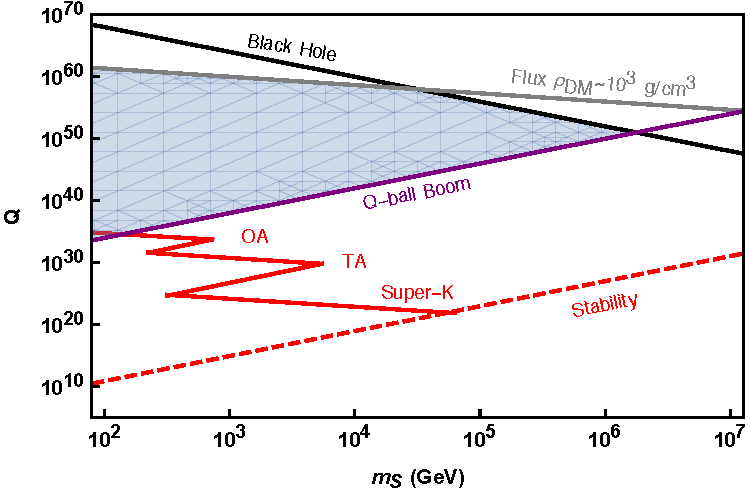
\includegraphics[scale=.55]{Qballconstraint.pdf}
\caption{Constraints on baryonic Q-balls from transits of a $\sim 1.25 ~M_{\odot}$ WD in the galactic center, $\rho_\text{DM} \sim 10^3 ~\text{g}/\text{cm}^3$. Also shown are the limits from Super-K and the OA, TA cosmic ray detectors.}
\label{fig:Qballconstraint}
\end{figure}

\section{Discussion}
\label{sec:Discussion}

It is clear that the detection of ultra-heavy DM is an open problem which will likely require a confluence of astrophysical probes.
Here we present a comprehensive guide to how white dwarfs can constrain such DM candidates that annihilate, decay, or transit a WD and release sufficient energy to trigger type Ia supernovae. 
In particular, we calculate the energy loss of high-energy particles due to SM interactions within the WD medium and determine the conditions for which a general energy deposition will heat a WD to the critical size and temperature necessary for thermonuclear runaway. 
As a concrete example we are able to place bounds on supersymmetric Q-ball DM over a wide region of parameter space, although the formalism provided will enable WDs to be applied as detectors for any DM models capable of heating the star through non-gravitational interactions. 
In general, the phenomenology of such a DM-induced event will be the ignition of sub-Chandrasekhar mass progenitors.
This raises the tantalizing possibility that DM encounters with a WD can act as an alternative explosion mechanism and progenitor system for type Ia SN. 
For decades, the standard lore has been that type Ia SN were due to the thermonuclear explosion of accreting carbon-oxygen white dwarfs in a binary system that reached the critical $\sim 1.4 ~M_{\odot}$ Chandrasekhar mass limit. 
Since the Chandrasekhar mass is a value determined only by fundamental physics it is natural to expect that the properties of type Ia SN are independent of initial conditions, famously enabling their use as ideal standard candles for precision luminosity distance measurements. 
However, it is well-known that such a mechanism cannot account for all observed type Ia SN. 
In fact, recent observations \cite{Scalzo:2014sap, Scalzo:2014wxa} suggest that an $\OO(1)$ fraction of the observed type Ia SN appear to have sub-Chandrasekhar progenitors.
The leading explanation for this phenomenon is the detonation of a surface layer of helium which drives a shock into the interior of a sub-Chandrasekhar-mass WD \cite{Woosley1994,Fink:2007fv}. 
In light of the lack of understanding of DM and its interactions, it is worthwhile to consider whether a DM-WD encounter may play the role of type Ia SN progenitor.


\begin{appendices}

\section{Particle Interactions in a White Dwarf}
\label{sec:Appendix}
Here we provide a detailed analysis of the electromagnetic and strong interactions in a WD.
This is primarily aimed towards calculating the stopping of electrons, photons, and light hadrons (pions, protons, neutrons) within the stellar medium at energies greater than $\sim \text{MeV}$.
These results of these stopping powers are summarized in Figures \ref{fig:SPelectron}, \ref{fig:SPphoton}, \ref{fig:SPnuc}, and \ref{fig:SPpion}.
Note that we will assume a carbon-oxygen WD.
The stellar medium is very dense, with electron and ion number densities in the range $n_e = Z n_\text{ion} \sim 10^{31} - 10^{33} ~\cm^{-3}$.
Such high densities will give rise to qualitatively different effects than seen in terrestrial detectors.
Famously, the star is supported against collapse by the relativistic electron degeneracy pressure with a characteristic Fermi energy
\begin{equation}
  E_F \sim (3 \pi^2 n_e)^{1/3} \sim 0.1 - 1 ~\MeV,
\end{equation}
which is greater than the typical stellar temperature $T \sim \keV$.
The nuclei are fully-ionized and form a strongly-coupled plasma with Coulomb interaction energy
\begin{equation}
\label{eq:lattice}
  \omega \sim \frac{Z^2 \alpha}{n_\text{ion}^{-1/3}}
         \sim 10^{-2} - 10^{-1} ~\MeV.
\end{equation}
Since it is generally the case that $\omega \gg T$, the ions form a Coulomb lattice with lattice binding energy $\sim \omega$.
\begin{figure}
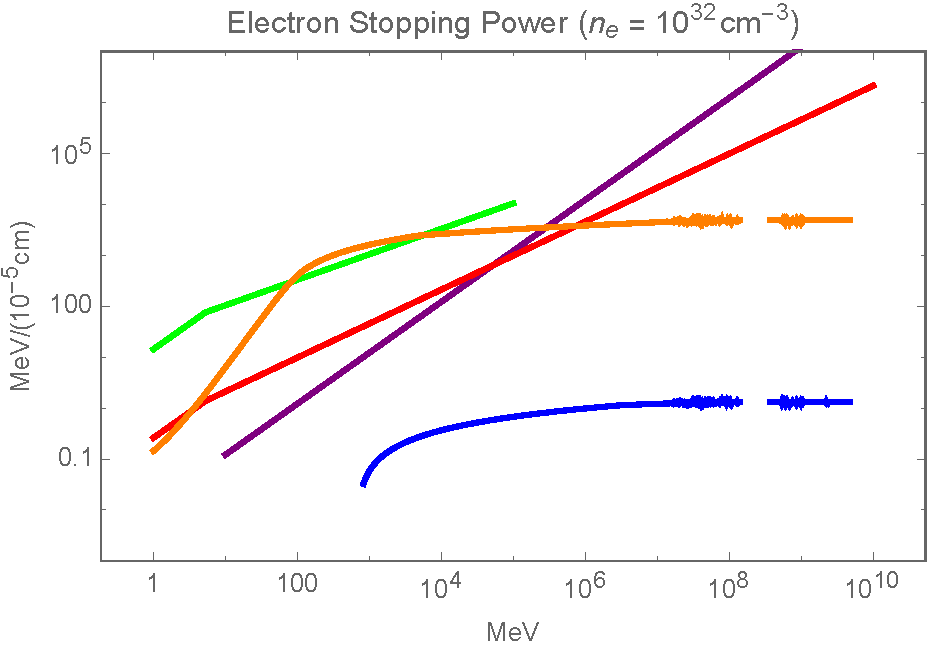
\includegraphics[scale=.60]{SPelectron.pdf}
\caption{Electron energy loss in a WD density $n_e = 10^{33} ~\text{cm}^{-3}$}
\label{fig:SPelectron}
\end{figure}

\begin{figure}
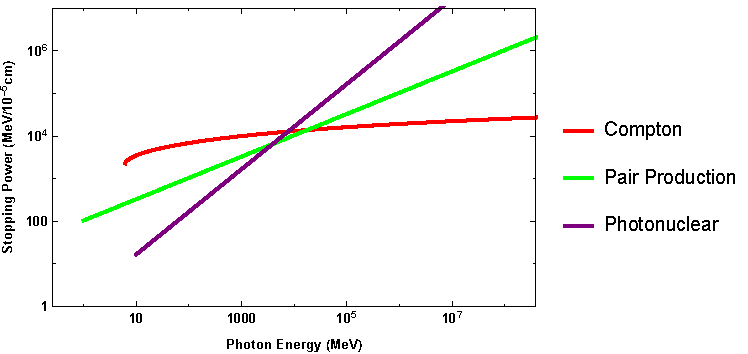
\includegraphics[scale=.60]{SPphoton.pdf}
\caption{Photon energy loss in a WD density $n_e = 10^{33} ~\text{cm}^{-3}$}
\label{fig:SPphoton}
\end{figure}

\begin{figure}
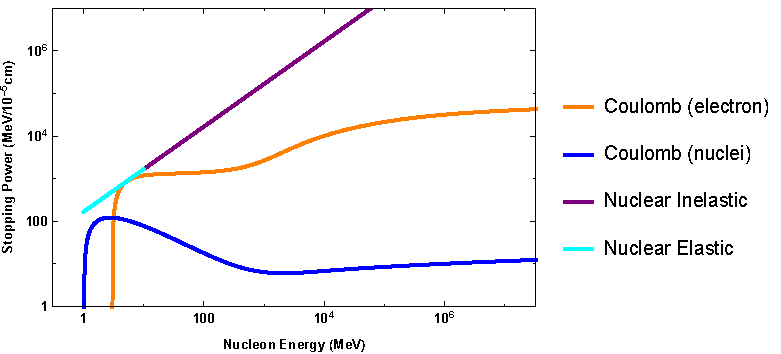
\includegraphics[scale=.60]{SPnucleon.pdf}
\caption{Nucleon energy loss in a WD with density $n_e = 10^{33} ~\text{cm}^{-3}$. The Coulomb stopping powers apply only to protons.}
\label{fig:SPnuc}
\end{figure}

\begin{figure}
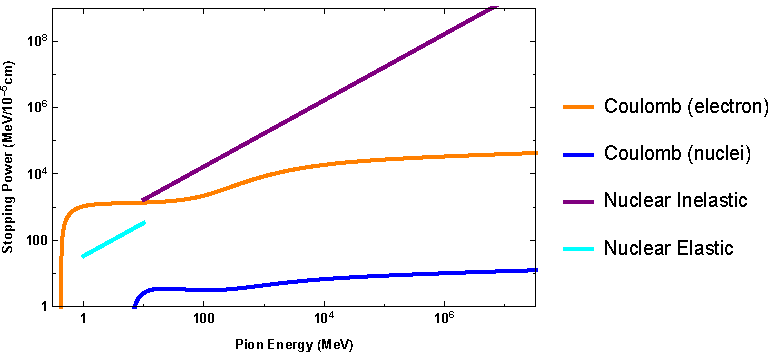
\includegraphics[scale=.60]{SPpion.pdf}
\caption{Pion energy loss in a WD with density $n_e = 10^{33} ~\text{cm}^{-3}$. The Coulomb stopping powers apply only to charged pion.}
\label{fig:SPpion}
\end{figure}

\subsection{Coulomb Collisions}
A particle of mass $m$, charge $e$, and velocity $\beta$ incident on a stationary target of mass $M$ and charge $Ze$ will transfer an energy $W$ as given by the recoilless Mott cross-section
\begin{equation}
  \frac{d \sigma}{dW} = \frac{2 \pi  Z^2 \alpha^2}{M \beta^2} \frac{1}{W^2}
    \l 1-\beta^2 \frac{W}{W_\text{kin}} \r,
\label{eq:mott}
\end{equation}
and we have assumed a sufficiently fast incident particle so that interactions are governed by single collisions with energy transfer $W$.
$W_\text{kin}$ is the maximum possible energy transfer satisfying kinematic constraints (i.e., a backward scatter)
\begin{equation}
\label{eq:ekin}
  W_{\text{kin}} = \frac{2 M \beta^2 \gamma^2}{1+ 2\gamma M/m +(M/m)^2}.
\end{equation}
It is straightforward to understand the parametric dependences of \eqref{eq:mott}: there is increased likelihood to scatter for slowly moving incident particles undergoing soft-scatters against lighter targets.
However, since we are ultimately interested in the transfer of energy to ions in the WD, we will consider the Coulomb energy loss to both nuclei and electron targets.

We first compute the stopping power due to scattering off nuclei, which is parametrically of the form
\begin{align}
\label{eq:SP}
  - \l \frac{dE}{dx}\r \sim \frac{2 \pi n_\text{ion} Z^2 \alpha^2}{M \beta^2}
    \log {\l\frac{W_\text{kin}}{W_\text{min}}\r}.
\end{align}
The minimum energy transfer $W_\text{min}$ is set by either charge screening or lattice effects.
In a WD, the screening length $\kappa_{\text{sc}}^{-1}$ due to the degenerate electron gas can be calculated in the Thomas-Fermi approximation \cite{Teukolsky}
\begin{equation}
\label{eq:TF}
\kappa_{\text{sc}}^{2} = \frac{6 \pi \alpha n_e}{E_F}.
\end{equation}
To estimate the energy transfer at this screening length, we use the fact that a soft Coulomb scatter at impact parameter $b$ will transfer energy of order
\begin{equation}
\label{eq:impact}
  W \sim \frac{Z^2 \alpha^2}{b^2 \beta^2 M}.
\end{equation}
In addition, for energy transfers less than the binding energy $\omega$, the lattice structure of ions must be taken into account.
Since the binding energy is much greater than the energy transfer set by screening, we take the lower-bound on free-particle Coulomb scattering to be $W_\text{min} \sim \omega$, only applicable in the case of nuclear targets.
However, doing so we find that the stopping power of electron-nuclei scattering vanishes at an incident energy $\sim 10 - 100 ~\MeV$ when the kinematic limit $W_\text{kin}$ becomes of order the binding energy $\omega$.
A similar cutoff occurs in the stopping of heavy charged hadrons (i.e., protons and pions), although in this energy range strong interactions will be a more dominant source of energy loss to nuclear targets anyway.
For low energy transfers $W < \omega$, we estimate the stopping power of electrons by considering the cross-section to scatter into phonon excitations of the lattice.

We now turn to computing the stopping power due to collisions with electrons targets.
In this case, electron degeneracy plays a significant role as an incident particle transferring energy $W$ can only scatter electrons within $W$ of the Fermi surface.
Although one must consider the relativistic velocities of the degenerate electrons, to leading order we simply average over this motion and treat the targets as stationary.
To account for degeneracy we define a modified number density of electrons in the WD
\begin{equation}
\label{eq:pauliblocking}
  n_e \l W \r =
  \begin{cases}
    \displaystyle \int \limits_{E_F - W}^{E_F} dE ~g(E), &  W < E_F  \\
    \quad             n_e                                &  W > E_F,
  \end{cases}
\end{equation}
where $g(E)$ is the density of states per unit volume of a three-dimensional free electron gas.
Therefore, unlike in the non-degenerate case, the energy loss from soft-scatters are in fact subdominant to the contributions from rare hard-scatters.
For an incident electron, we additionally demand that the energy remains above the Fermi surface after scattering, $W < E - E_F$.
Note that \eqref{eq:mott} is no longer fully valid in the case of electron-electron scattering due to the significant target recoil as well as identical particle effects, and a more accurate calculation requires the M{\"o}ller cross-section.
Nevertheless, at sufficiently high energies the stopping power for all charged particles scattering off electrons is roughly constant and of order
\begin{equation}
-\l \frac{dE}{dx} \r \sim \frac{2 \pi n_e \alpha^2}{m_e}.
\end{equation}
However, the low-energy behavior is not so straightforward due to the effects of Pauli-blocking and charge screening.
In every case, we find that the stopping power decreases with incident energy until a critical threshold is reached where screening effectively cuts off the energy loss.

\subsubsection{Phonon production}

To describe the contribution of phonons to the Coulomb scattering stopping power, we will calculate an approximate dynamic structure factor describing the white dwarf lattice. It is sufficient for our purposes to approximate the vibrational response of the white dwarf as a collection of harmonic oscillators at the plasma frequency
\begin{align}
\Omega_p = \sqrt{\frac{4 \pi n_i Z^2 \alpha}{M}} \sim 1 - 10~\text{keV}
\end{align}
where $M$ is the mass of carbon. (Note that the Debye temperature in a white dwarf is equal to its plasma frequency. \cite{reference}) We will assume that the white dwarf has temperature $T\lesssim 1~\text{keV}$ so that the temperature is low compared to the phonon energies. \textcolor{blue}{This is a typical white dwarf temperature \cite{reference}.}

The doubly differential cross section (see, for instance \textcolor{blue}{[Kittel]}) is given by
\begin{align}
\frac{d^2 \sigma}{d \Omega\, d \omega} = \frac{k'}{k} \left( \frac{m}{2 \pi} \right)^2 |V_\textbf{q}|^2 S(\textbf{q}, \omega)
\label{eq:DoublyDifferentialCrossSection}
\end{align}
where $V_\textbf{q}$ is the fourier transform of the interaction potential and $S(\textbf{q}, \omega)$ is the dynamic structure factor. Here $\omega$ is the energy transferred to the target particle, $m$ is the mass of the incident particle, and $k$ and $k'$ are the initial and final momentum of the incident particle, respectively. This is a non-relativistic formalism, and while we may restrict ourselves to non-relativistic targets, any incident electrons of interest will be relativistic. Conveniently, however, we note that if we use the free particle structure factor $S(\textbf{q}, \omega) = \delta(\omega - q^2 / 2 M)$ we can recover exactly the first term of the proper relativistic result~\eqref{eq:mott} by simply making the substitution $m^2 / k^2\to 1/\beta^2$. This same factor appears in the phonon calculation we need, so we will make the same substitution and use this as an approximation for the proper relativistic result.

The structure factor for a single harmonic oscillator with frequency $\omega_0$ at temperatures $T\ll \omega_0$ is (e.g., \cite{reference})
\begin{align}
S(\textbf{q}, \omega) &= e^{-q^2 / 2 M \omega_0} \bigg[ \delta(\omega) + \frac{q^2}{2 M \omega_0}\delta(\omega - \omega_0)\nonumber\\
&\qquad + \frac12 \left( \frac{q^2}{2 M \omega_0} \right)^2 \delta(\omega - 2\omega_0) + \cdots \bigg]
\label{eq:HarmonicOscillatorStructureFactor}
\end{align}
The first term encodes an elastic scatter, the second a 1-phonon process, the third a 2-phonon process, etc. We are only interested in the inelastic pieces which may transfer energy to the ions. As we should expect, equation~\eqref{eq:HarmonicOscillatorStructureFactor} approaches the structure factor for a free particle at large energy transfers $\omega \gg \omega_0$, and accordingly we should expect the stopping powers to match when the incident energy is so large that even the free particle stopping power is dominated by energy transfers above the plasma frequency. \textcolor{blue}{(Where is this, and how do we see it?)}

The interaction potential between an incident particle with charge $\pm 1$ and a carbon ion is given by
\begin{align}
V_\textbf{q} = \frac{4 \pi Z\alpha}{q^2 + \lambda_T^2}
\label{eq:InteractionPotential}
\end{align}
where $\lambda_T$ is the Thomas-Fermi screening length. Inserting equations~\eqref{eq:HarmonicOscillatorStructureFactor} and~\eqref{eq:InteractionPotential} into~\eqref{eq:DoublyDifferentialCrossSection}, integrating over solid angle with a relativistic incident particle, and making the substitution $m^2 / k^2\to 1/\beta^2$ discussed earlier, we find the cross section per unit energy transfer for a $n$-phonon process to be
\begin{align}
\frac{d \sigma_n}{d \omega}&= \frac{2 \pi Z^2 \alpha^2}{M\beta^2 \omega_0^2} \delta(u - n) g_n(u)
\end{align}
with the dimensionless function
\begin{align}
  g_n(u) &= \int_{Q_1^2}^{Q_2^2} d(Q^2)\, \frac{e^{-Q^2}}{(Q^2 + \eta^2)^2} \frac{(Q^2)^n}{n!}
\end{align}
where $Q_1^2 = u^2 \omega_0 / 2 M$ and $Q_2^2 = (2 \kappa - u)^2 \omega_0 / 2 M$, and we have defined the dimensionless variables $u = \omega / \omega_0$, $\kappa = k / \omega_0$, and $\eta^2 = \lambda^2 / 2 M \omega_0$.

To compute the stopping power for an electron scattering off ions, we sum the contributions from all possible phonon processes and integrate over all energy transfers that would keep the electron above the Fermi sea:
\begin{align}
-\frac{dE}{dx} &= \int_0^{k - E_f} d\omega\, n_\text{ion}\omega_0\sum_{n = 1}^{\infty} \frac{d \sigma_n}{d \omega} \nonumber\\
 &= \frac{2 \pi n_\text{ion} Z^2 \alpha^2}{M \beta^2} \sum_{n = 1}^{n_\text{max}} g_n(n)
 \label{eq:PhononStoppingPower}
\end{align}
where $n_\text{max} = (k - E_f) / \omega_0$. One can easily check numerically that the sum is within 10\% of the Coulomb logarithm for the free particle calculation, so we have found that the free particle and phonon stopping powers \eqref{eq:SP} and \eqref{eq:PhononStoppingPower} are the same, and we can simply continue the free particle stopping power curve all the way down to the Fermi energy where it must cut off for degeneracy reasons anyways.

\textcolor{blue}{omit this paragraph?} It is interesting that even though the phonon and free particle results have different total cross-sections and different typical energy transfers---free particle scatters are dominated by transfers of $ \sim 10^{-7}~\text{MeV}$ near the screen length, whereas phonon excitations are dominated by 1-phonon processes transferring $ \sim 10^{-2}~\text{MeV}$---these are just properly balanced so that the stopping powers come out the same. This would not be remarkable if the scattering were dominated by hard scatters, so that single-phonon processes were negligible, but we might not expect this of a process dominated by soft scatters. This seems to be a coincidence of the Coulomb interaction, and we would not expect to see this for interactions that drop off faster than $1 / r$.

% \log {\l\frac{W_\text{kin}}{W_\text{min}}\r}

 \subsection{Compton and Inverse Compton Scattering}

Photons and charged particles can elastically exchange energy through Compton scattering.
We focus first on an incident photon losing energy to the WD medium.
Since the cross-section for this process scales inversely with the target mass, the stopping due to photon-ion collisions will be far subdominant to photon-electron collisions and we ignore the former.
Consider an incident photon of energy $k$ scattering off an electron of energy $\sim E_F$.
In the rest frame of the electron, this cross-section is given by the Klein-Nishina formula
\begin{equation}
\label{KN}
  \frac{d\sigma_\text{KN}}{d (\cos \theta)} = \frac{\pi \alpha^2}{m_e^2}
  \l \frac{k^\prime}{k} \r^2
  \l \frac{k^\prime}{k} + \frac{k}{k^\prime} -\sin^2 \theta \r
\end{equation}
where $k^\prime$ is the outgoing photon energy, related to the scattering angle $\theta$ by the Compton formula
\begin{equation}
{k^{\prime }={\frac {k}{1+{\frac {k}{m_e}}(1-\cos \theta )}}}.
\end{equation}
In the limit $k > m_e$, the cross-section is suppressed by the incoming energy $\sigma_\text{KN} \sim \frac{\alpha^2}{m_e k}$.
The outgoing photons will scatter predominately in a near-forward direction $\cos \theta \approx m_e/k$ so that $k^\prime \sim m_e$.
Thus the typical photon energy loss is large, and cooling proceeds via a small number of hard scatters.
The Compton stopping power is estimated to be
\begin{equation}
\label{eq:approx-comptonSP}
  - \l\frac{dk}{dx}\r \sim \frac{n_e \alpha^2}{m_e} \l 1 - \frac{m_e}{k} \r.
\end{equation}
A more detailed analysis computes the stopping power as
\begin{equation}
\label{eq:comptonSP}
  -\l\frac{dk}{dx}\r =  \int d (\cos \theta) n_e \frac{d\sigma_\text{KN}}{d (\cos \theta)} \l k - k^\prime \r,
\end{equation}
with an appropriate Lorentz boost to the electron rest frame, although the full result only differs from the above estimate by $\OO(1)$ factors.
Further, Pauli-blocking of the target electrons is taken into account using a modified number density as in \eqref{eq:pauliblocking}.
We find that degeneracy only introduces a significant suppression when $k \lesssim 10 ~\text{MeV}$, which is to be expected since the interaction is dominated by hard, near-forward scatters.

We now briefly consider incident electrons which may cool by inverse Compton scatters with the thermal bath of photons in the WD.
The number density of these photons is set by the temperature of the star $n_\gamma \sim T^3 \sim 10^{23} ~\cm^{-3}$, where we have taken $T \sim \text{keV}$.
As this is parametrically smaller than the number density of electrons, it is reasonable to suspect that the energy loss due to inverse Compton scattering is far subdominant to electron-electron collisions.
An estimate in the manner of \eqref{eq:approx-comptonSP} gives the inverse Compton stopping power in terms of the photon temperature $T$ and incident electron energy $E$
\begin{equation}
\label{eq:invcomptonSP}
  -\l \frac{dE}{dx}\r \sim
  \begin{cases}
    \alpha^2 \frac{T^4}{m_e^4} E^2 & E \lesssim \frac{m_e^2}{T} \\
    \alpha^2 T^2 & E \gtrsim \frac{m_e^2}{T} \\
  \end{cases},
\end{equation}
where the change in scaling with $E$ marks a transition from Thompson-like scattering in the electron rest frame to suppressed high-energy scattering.
As expected, we find that the inverse Compton stopping power is negligible compared to Coulomb scattering.

\subsection{Bremsstrahlung and Pair Production with LPM Suppression}

Bremsstrahlung and pair production can be a dominant stopping mechanisms for high-energy electrons and photons.
We restrict our attention to radiative processes off target nuclei rather than target electrons as the latter are additionally suppressed by degeneracy, kinematic recoil, and charge factors.
The cross-section for an electron of energy $E$ to radiate a photon of energy $k$ is given by the Bethe-Heitler formula
\begin{equation}
\label{eq:BH}
\frac{d \sigma_\text{BH}}{dk} = \frac{1}{3 k n_\text{ion} X_0} (y^2+2 [1+ (1-y)^2]), ~~~ y = k/E.
\end{equation}
$X_0$ is the radiation length, and is generally of the form
\begin{equation}
\label{eq:radiationlength}
X_0^{-1} = 4 n_\text{ion} Z^2 \frac{\alpha^3}{m_e^2} \log{\Lambda}, ~~~ \log{\Lambda} \sim \int \frac{1}{b}.
\end{equation}
where $\log{\Lambda}$ is a logarithmic form factor containing the maximum and minimum effective impact parameters allowed in the scatter.
Integrating \eqref{eq:BH}, we find the energy loss due to bremsstrahlung is simply
\begin{equation}
-\l\frac{dE}{dx}\r \sim \frac{E}{X_0}.
\end{equation}
In \eqref{eq:radiationlength}, the minimum impact parameter is set by a quantum-mechanical bound such that the radiated photon frequency is not larger than the initial electron energy.
For a bare nucleus, this distance is the electron Compton wavelength.
It is important to note that collisions at lesser impact parameters will still radiate but with suppressed intensity.
The maximum impact parameter is set by the distance at which the nuclear target is screened.
For an atomic target this is of order the Bohr radius, and for nuclear targets in the WD this is the Thomas-Fermi screening radius given by \eqref{eq:TF}.
%Evidently, there exists a critical electron number density $n_e \sim 10^{32} ~\text{cm}^{-3}$ for which the logarithmic form factor appears to vanish.
For our purposes, we simply take $\log{\Lambda} \sim \OO(1)$ for all WD densities under consideration and refrain from a full quantum-mechanical calculation at small impact parameters.

However, bremsstrahlung will be suppressed by the ``Landau-Pomeranchuk-Migdal" (LPM) effect - see \cite{Klein:1998du} for an extensive review.
High-energy radiative processes involve very small longitudinal momentum transfers to nuclear targets ($\propto k/E^2$ in the case of bremsstrahlung).
Quantum mechanically, this interaction is delocalized across a formation length over which amplitudes from different scattering centers will interfere.
This interference turns out to be destructive and must be taken into account in the case of high energies or high-density mediums.
Calculations of the LPM effect can be done semi-classically based on average multiple scattering.
It is found that bremsstrahlung is suppressed for $k < E(E-k)/E_\text{LPM}$, where
\begin{equation}
\label{eq:LPM}
E_\text{LPM} = \frac{m_e^2 X_0 \alpha}{4 \pi}.
\end{equation}
For the WD densities in which radiative energy loss is considered, $E_\text{LPM} \sim 1-10^{2} ~\text{MeV}$.
The degree of suppression is found to be
\begin{equation}
\frac{d\sigma_\text{LPM}/dk}{d\sigma_\text{BH}/dk} = \sqrt{\frac{k E_\text{LPM}}{E (E-k)}},
\end{equation}
so that the bremsstrahlung stopping power in the regime of high-suppression is modified
\begin{equation}
\label{eq:bremloss}
-\l\frac{dE}{dx}\r_\text{LPM} \sim \l\frac{E_\text{LPM}}{E} \r^{1/2} \frac{E}{X_0}, ~~~ E>E_\text{LPM}.
\end{equation}
We find that the LPM effect diminishes energy loss due to soft radiation so that the radiative stopping power is dominated by single, hard bremsstrahlung.

In addition to the LPM effect, other forms of interaction within a formation length will suppress bremsstrahlung when $k \ll E$.
The emitted photon can coherently scatter off electrons and ions in the media, acquiring an effective mass of order the plasma frequency $\omega_p$.
Semi-classically, this results in a suppression of order $(k/\gamma \omega_p)^2$ when the radiated photon energy $k < \gamma \omega_p$.
This is known as the ``dielectric effect".
For high-energy electrons, this dielectric suppression only introduces a minor correction to \eqref{eq:bremloss}, in which soft radiation is already suppressed by the LPM effect \cite{Klein:1998du}.

We now briefly summarize the stopping of photons via pair production. Similar to \eqref{eq:BH}, the cross-section for a photon of energy $k$ to produce an electron-positron pair with energies $E$ and $k-E$ is
\begin{equation}
\label{eq:PP}
\frac{d \sigma_\text{BH}}{dE} = \frac{1}{3 k n_\text{ion} X_0} (1+ 2[x^2+ (1-x)^2]) ~~~ x = E/k,
\end{equation}
valid beyond the threshold energy $k \gtrsim m_e$.
As a result, the pair production cross-section $\sim 1/(n_\text{ion} X_0)$.
However, the LPM effect suppresses pair production at energies $E(k-E) > k E_\text{LPM}$ so that the cross-section reduces to
\begin{equation}
\sigma_{pp} \sim \l\frac{E_\text{LPM}}{k} \r^{1/2} \frac{1}{n_\text{ion} X_0}, ~~~ E>E_\text{LPM}.
\end{equation}
Note that the LPM effect is less significant for higher-order electromagnetic processes since these generally involve larger momentum transfers for the same final-state kinematics.
Thus, when the suppression factor exceeds $\OO(\alpha)$, these interactions should also be considered.
For instance, the energy loss due to electron direct pair production $eN \to e^+ e^- e N$ has been calculated in \cite{Gerhardt:2010bj} and is found to exceed that of bremsstrahlung at an energy $\sim 10^{8} ~\GeV$.
A similar crossover is to be expected for other higher-order diagrams as well, although such a calculation is beyond the scope of this work.
Rather, at such high energies the stopping power is dominated by photonuclear and electronuclear interactions anyway, and we may simply ignore the contributions from other radiative processes \cite{Kleinconvo}.

\subsection{Nuclear Interactions}

Nuclear interactions can be either elastic or inelastic - the nature of the interaction is largely determined by the incident particle energy.
Elastic collisions are most significant for energy loss at scales less than the nuclear binding energy $\sim 10 ~\text{MeV}$.
A single, backward elastic scatter could result in an incident particle losing virtually all of its energy if the incident and target masses are the same.
However, we will be primarily concerned with light hadrons incident on relatively heavy nuclei, i.e. ping-pong balls bouncing around a sea of bowling balls.
An elastic collision between a incident, non-relativistic hadron of mass $m$, kinetic energy $E$ and a stationary nuclear target of mass $M$ results in an average final energy
\begin{equation}
\label{eq:elasticratio}
E' \sim \l \frac{m}{M}\r E, ~~~~ m < M,
\end{equation}
where it is assumed there is an isotropic distribution in the center-of-mass scattering angle.
Above $\sim \text{MeV}$, it is found that electrostatic repulsion is negligible for nuclear interactions of protons and $\pi^+$.
Therefore, the stopping power for any light hadron due to elastic collisions is of the form
\begin{equation}
- \l \frac{dE}{dx} \r \sim \l \frac{m}{M} \r \frac{E}{l_\text{el}}.
\end{equation}
$l_\text{el}$ denotes the mean free path for elastic collisions characterized by cross-section $\sigma_\text{el}$.
Above $10 ~\MeV$ the nuclear elastic cross-section approaches the geometric cross-section for carbon $\sim 100 ~\text{mb}$, while at $\MeV$ energies the elastic cross section generally rises to be of order $\sim \text{b}$.
At intermediate energies $1 - 10 ~\MeV$, the interaction is dominated by various nuclear resonances.
For our purposes, we will conservatively estimate the elastic cross section for nucleons and pions to be $\sigma_\text{el} \approx 1 ~\text{b}$ when $E \lesssim 10 ~\MeV$, and ignore the energy loss due to elastic scatters at higher energies where inelastic processes will dominate.

Now we determine the stopping power due to inelastic nuclear collisions at $E \gtrsim 10 ~\MeV$.
In such a collision, an incoming hadron interacts with one or more nucleons in the nucleus to produce a $\OO(1)$ number of additional hadrons which approximately split the initial energy.
For incident energies greater than the nucleon binding energy $\sim \GeV$, the secondary hadrons are mostly pions which carry transverse momentum of order $\sim 100 ~\MeV$.
In addition, during this process the target nucleus is broken up.
The nuclear fragment is typically left in an unstable state with negligible center-of-mass recoil, and relaxes via the slow emission of low-energy $\sim \MeV$ hadrons and photons.
Note that for incident hadrons in the range $10 ~\MeV - \GeV$, it is found that roughly equal fractions of protons, neutrons, and pions are emitted after each inelastic collision.
In either case, if secondary hadrons are sufficiently energetic then they will induce further inelastic collisions.
A roughly collinear hadronic shower is the result of all such interactions caused by primary and secondary particles.
This cascade is adequately described by a radiative stopping power
\begin{equation}
\label{eq:nucshower}
-\l \frac{dE}{dx}\r \sim \frac{E}{l_\text{inel}},
\end{equation}
neglecting of $\OO(1)$ logarithmic factors.
$l_\text{inel}$ is the inelastic nuclear mean free path characterized by an inelastic cross-section $\sigma_\text{inel}$.
At these energies, $\sigma_\text{inel} \approx 100 ~\text{mb}$ and is roughly constant in energy.
The shower will end once final-state hadrons reach a critical energy - this is either the scale at which an additional mechanism dominates the stopping power or the nuclear binding energy $\sim 10 ~\MeV$.

Photons of energy $k \gtrsim 10 ~\text{MeV}$ can also strongly interact with nuclei through the production of virtual quark-antiquark pairs.
Photonuclear interactions are similar in nature to the inelastic collisions of hadrons, although the cross-section $\sigma_{\gamma A}$ is roughly a factor $\approx \alpha$ smaller.
Below $\sim \GeV$ the photonuclear cross-section is complicated by nuclear resonances while above $\sim \GeV$, $\sigma_{\gamma A}$ is a slowly increasing function of energy.
At sufficiently high energies, photonuclear interactions can in fact become coherent with the photon interaction spread over multiple nuclei \cite{Gerhardt:2010bj}.
This coherence will further reduce the photonuclear mean free path $l_{\gamma A}$.
As a conservative estimate, at energies $k \gtrsim 10 ~\text{MeV}$ we assume a constant photonuclear cross-section of order $\sigma_{\gamma A} \approx \text{mb}$.
Similarly, electrons can also lose energy by radiating a virtual photon that interacts hadronically with a nearby nucleus.
Naively we would expect the electronuclear stopping power to parametrically be of the form $(dE/dx) \sim E \alpha/l_{\gamma A}$.
A more detailed calculation in \cite{Gerhardt:2010bj} obtains a similar result but with an additional $\OO(10)$ numerical factor.
\end{appendices}

\section*{Acknowledgements}
We would like to thank Dorota Grabowska, Keisuke Harigaya, Spencer Klein, Jacob Leedom, Robert McGehee, Lian-Tao Wang, and Jonathan Wurtele for stimulating discussions.
\textcolor{blue}{Grant acknowledgements}

\begin{thebibliography}{99}
\bibliographystyle{unsrt} 

\bibitem{Graham:2015apa} 
  P.~W.~Graham, S.~Rajendran and J.~Varela,
  %``Dark Matter Triggers of Supernovae,''
  Phys.\ Rev.\ D {\bf 92}, no. 6, 063007 (2015)
  %doi:10.1103/PhysRevD.92.063007
  [arXiv:1505.04444 [hep-ph]].
  
\bibitem{Gasques:2005ar} 
  L.~R.~Gasques, A.~V.~Afanasjev, E.~F.~Aguilera, M.~Beard, L.~C.~Chamon, P.~Ring, M.~Wiescher and D.~G.~Yakovlev,
  %``Nuclear fusion in dense matter: Reaction rate and carbon burning,''
  Phys.\ Rev.\ C {\bf 72}, 025806 (2005)
  %doi:10.1103/PhysRevC.72.025806
  [astro-ph/0506386].
  
\bibitem{Woosley}
 F.~X. Timmes and S.~E. Woosley, Astro. Phys. Journal {\bf 396}, 649 (1992).
 
\bibitem{Tavernier}
S.~Tavernier, "Experimental Techniques in Nuclear and Particle Physics", Springer (2010). 
 
\bibitem{Teukolsky}
S.~L.~Shapiro and S.~A.~Teukolsky, ``Black Holes, White Dwarfs, and Neutron Stars", Wiley (1983).

\bibitem{Chandrasekhar}
S.~Chandrasekhar, ``An Introduction to the Study of Stellar Structure", University of Chicago press (1939).

\bibitem{Rossi}
B.~Rossi, ``High Energy Particles", Prentice-Hall, Inc., Englewood Cliffs, NJ (1952). 

\bibitem{Coleman:1985ki} 
  S.~R.~Coleman,
  %``Q Balls,''
  Nucl.\ Phys.\ B {\bf 262}, 263 (1985)
  Erratum: [Nucl.\ Phys.\ B {\bf 269}, 744 (1986)].

\bibitem{Kusenko:1997si} 
  A.~Kusenko and M.~E.~Shaposhnikov,
  %``Supersymmetric Q balls as dark matter,''
  Phys.\ Lett.\ B {\bf 418}, 46 (1998)
  %doi:10.1016/S0370-2693(97)01375-0
  [hep-ph/9709492].

\bibitem{Dine:2003ax} 
  M.~Dine and A.~Kusenko,
  %``The Origin of the matter - antimatter asymmetry,''
  Rev.\ Mod.\ Phys.\  {\bf 76}, 1 (2003)
  %doi:10.1103/RevModPhys.76.1
  [hep-ph/0303065].

\bibitem{Kasuya:2015uka} 
  S.~Kasuya, M.~Kawasaki and T.~T.~Yanagida,
  %``IceCube potential for detecting Q-ball dark matter in gauge mediation,''
  PTEP {\bf 2015}, no. 5, 053B02 (2015)
  %doi:10.1093/ptep/ptv056
  [arXiv:1502.00715 [hep-ph]].

\bibitem{Agashe:2014kda} 
  K.~A.~Olive {\it et al.} [Particle Data Group],
  %``Review of Particle Physics,''
  Chin.\ Phys.\ C {\bf 38}, 090001 (2014).
  %doi:10.1088/1674-1137/38/9/090001
  
\bibitem{Hardy:2014mqa} 
  E.~Hardy, R.~Lasenby, J.~March-Russell and S.~M.~West,
  %``Big Bang Synthesis of Nuclear Dark Matter,''
  JHEP {\bf 1506}, 011 (2015)
  %doi:10.1007/JHEP06(2015)011
  [arXiv:1411.3739 [hep-ph]].

\bibitem{Gerhardt:2010bj} 
  L.~Gerhardt and S.~R.~Klein,
  %``Electron and Photon Interactions in the Regime of Strong LPM Suppression,''
  Phys.\ Rev.\ D {\bf 82}, 074017 (2010)
  %doi:10.1103/PhysRevD.82.074017
  [arXiv:1007.0039 [hep-ph]].

\bibitem{Pionnuclear}
T.~S.~H.~Lee and R.~P.~Redwine,
 %``Pion-Nucleus Interactions", 
 Annu. Rev. Nucl. Part. Sci {\bf 52}, pp.23-63 (2002)

\bibitem{Formaggio:2013kya} 
  J.~A.~Formaggio and G.~P.~Zeller,
  %``From eV to EeV: Neutrino Cross Sections Across Energy Scales,''
  Rev.\ Mod.\ Phys.\  {\bf 84}, 1307 (2012)
  %doi:10.1103/RevModPhys.84.1307
  [arXiv:1305.7513 [hep-ex]].
  
\bibitem{Jackson}
J.~D.~Jackson, ``Classical Electrodynamics", 3rd edition, John Wiley and Sons, New
York, (1998).
 
 \bibitem{Klein:1998du} 
  S.~Klein,
  %``Suppression of Bremsstrahlung and pair production due to environmental factors,''
  Rev.\ Mod.\ Phys.\  {\bf 71}, 1501 (1999)
  %doi:10.1103/RevModPhys.71.1501
  [hep-ph/9802442].

\bibitem{AlvarezMuniz:1998px} 
  J.~Alvarez-Muniz and E.~Zas,
  %``The LPM effect for EeV hadronic showers in ice: Implications for radio detection of neutrinos,''
  Phys.\ Lett.\ B {\bf 434}, 396 (1998)
  %doi:10.1016/S0370-2693(98)00905-8
  [astro-ph/9806098].

\bibitem{Padmanabhan:2005es} 
  N.~Padmanabhan and D.~P.~Finkbeiner,
  %``Detecting dark matter annihilation with CMB polarization: Signatures and experimental prospects,''
  Phys.\ Rev.\ D {\bf 72}, 023508 (2005)
  %doi:10.1103/PhysRevD.72.023508
  [astro-ph/0503486].

\bibitem{Poulin:2016nat} 
  V.~Poulin, P.~D.~Serpico and J.~Lesgourgues,
  %``A fresh look at linear cosmological constraints on a decaying dark matter component,''
  JCAP {\bf 1608}, no. 08, 036 (2016)
  %doi:10.1088/1475-7516/2016/08/036
  [arXiv:1606.02073 [astro-ph.CO]].

\bibitem{Randall:2007ph} 
  S.~W.~Randall, M.~Markevitch, D.~Clowe, A.~H.~Gonzalez and M.~Bradac,
  %``Constraints on the Self-Interaction Cross-Section of Dark Matter from Numerical Simulations of the Merging Galaxy Cluster 1E 0657-56,''
  Astrophys.\ J.\  {\bf 679}, 1173 (2008)
  %doi:10.1086/587859
  [arXiv:0704.0261 [astro-ph]].
  
\bibitem{ThePierreAuger:2015rha} 
  A.~Aab {\it et al.} [Pierre Auger Collaboration],
  %``Measurement of the cosmic ray spectrum above 4 $\times$ 10$^{18}$ eV using inclined events detected with the Pierre Auger Observatory,''
  JCAP {\bf 1508}, 049 (2015)
  %doi:10.1088/1475-7516/2015/08/049
  [arXiv:1503.07786 [astro-ph.HE]].

\bibitem{AbuZayyad:2012ru} 
  T.~Abu-Zayyad {\it et al.} [Telescope Array Collaboration],
  %``The Cosmic Ray Energy Spectrum Observed with the Surface Detector of the Telescope Array Experiment,''
  Astrophys.\ J.\  {\bf 768}, L1 (2013)
  %doi:10.1088/2041-8205/768/1/L1
  [arXiv:1205.5067 [astro-ph.HE]].
  
\bibitem{Nesti:2013uwa} 
  F.~Nesti and P.~Salucci,
  %``The Dark Matter halo of the  Milky Way, AD 2013,''
  JCAP {\bf 1307}, 016 (2013)
  %doi:10.1088/1475-7516/2013/07/016
  [arXiv:1304.5127 [astro-ph.GA]].

\bibitem{Mereghetti:2013nba} 
  S.~Mereghetti,
  %``RX J0648.0--4418: the fastest-spinning white dwarf,''
  %doi:10.1142/9789814623995_0469
  arXiv:1302.4634 [astro-ph.HE].

\bibitem{cococubed}
F.~X.~Timmes, http://cococubed.asu.edu/code pages/coldwd.shtml
  
\bibitem{SDSS}
S.~J.~Kleinman, S. O. Kepler, D. Koester, I. Pelisoli  {\it et al.}, Astrophys. J. Suppl. {\bf 204}, article
id. 5, 14 pp. (2013)

\bibitem{NuStar}
K.~Perez, C.~J.~Hailey, F.~E.~Bauer, {\it et al.}, Nature {\bf 520}, 646 (2015)

\bibitem{Kleinconvo}
S.~Klein, private communication

\bibitem{Scalzo:2014wxa} 
  R.~A.~Scalzo, A.~J.~Ruiter and S.~A.~Sim,
  %``The ejected mass distribution of type Ia supernovae: A significant rate of non-Chandrasekhar-mass progenitors,''
  Mon.\ Not.\ Roy.\ Astron.\ Soc.\  {\bf 445}, no. 3, 2535 (2014)
  doi:10.1093/mnras/stu1808
  [arXiv:1408.6601 [astro-ph.HE]].
  
  \bibitem{Scalzo:2014sap} 
  R.~Scalzo {\it et al.} [Nearby Supernova Factory Collaboration],
  %``Type Ia supernova bolometric light curves and ejected mass estimates from the Nearby Supernova Factory,''
  Mon.\ Not.\ Roy.\ Astron.\ Soc.\  {\bf 440}, no. 2, 1498 (2014)
  doi:10.1093/mnras/stu350
  [arXiv:1402.6842 [astro-ph.CO]].
  
  \bibitem{Fink:2007fv} 
  M.~Fink, W.~Hillebrandt and F.~K.~Roepke,
  %``Double-detonation supernovae of sub-Chandrasekhar mass white dwarfs,''
  Astron.\ Astrophys.\ 
  [Astron.\ Astrophys.\  {\bf 476}, 1133 (2007)]
  doi:10.1051/0004-6361:20078438
  [arXiv:0710.5486 [astro-ph]].
  
  \bibitem{Woosley1994}
  %Sub--Chandrasekhar Mass Models for Type IA Supernovae
  S.~E.~Woosley and T.~A.~Weaver, Astrophysical Journal {\bf 423}, pp.371-379 (1994).
  

\end{thebibliography}

\end{document}
